\documentclass[oneside, 10pt, a4paper, twocolumn]{article}

\usepackage[small]{titlesec}
\usepackage{fancyhdr}
\usepackage{pdfpages}
\usepackage{textcomp} 
\usepackage{amssymb}
\usepackage{amsmath}
\usepackage{amsthm}
\usepackage{amscd}
\usepackage{amsfonts}
\usepackage{mathrsfs}
\usepackage{graphicx}
\usepackage[utf8]{inputenc}
\usepackage[T1]{fontenc}
\usepackage[english]{babel}
\usepackage{color}
\usepackage{braket}
\usepackage{caption}  %tabelle
\usepackage{minitoc}
\usepackage{lmodern}
\usepackage{microtype}  %migliora scrittura
\usepackage{booktabs}  %tabelle
\usepackage{epsf}
\usepackage{epstopdf}
\usepackage{bm}
\usepackage{pdflscape}
\usepackage{varioref}
\usepackage{cite}
\usepackage{authblk}
\usepackage[columnwise, switch]{lineno}
\usepackage{authblk}
\usepackage[numbers]{natbib}
\usepackage{mwe}    % loads »blindtext« and »graphicx«
\usepackage{subfig}

%\usepackage{natbib}

%\usepackage[pagebackref]{hyperref}

%\linenumbers
\makeindex
\DeclareGraphicsExtensions{.jpg, .pdf, .png}

\renewcommand{\floatpagefraction}{.9}

\providecommand{\keywords}[1]{\textbf{Keywords:} \textit{#1}}

\makeindex

\begin{document}

\title{Supplementary Material of: Data-driven dynamical model indicates that the heat shock response in \emph{Chlamydomonas reinhardtii} is {tailored to handle} natural temperature variation}

\author[1,2]{Stefano Magni}
\author[3,5]{Antonella Succurro}
\author[2,4]{Alexander Skupin}
\author[1,5,$\dagger$]{Oliver Ebenhöh}
%\footnote{To whom correspondence should be addressed. E-mail: oliver.ebenhoeh@hhu.de}

\affil[1]{\small{Institute of Quantitative and Theoretical Biology, Heinrich Heine University, Düsseldorf, Germany}}
\affil[2]{\small{Luxembourg Centre for Systems Biomedicine, University of Luxembourg, Esch-sur-Alzette, Luxembourg}}
\affil[3]{\small{Botanical Institute, University of Cologne, Cologne, Germany}}
\affil[4]{\small{University California San Diego, La Jolla, USA}}
\affil[5]{\small{Cluster of Excellence on Plant Sciences (CEPLAS), Düsseldorf, Germany}}
%\affil[1]{\small{Institute for Quantitative and Theoretical Biology, Heinrich Heine University Düsseldorf, Germany}}
%\affil[2]{\small{Luxembourg Centre for Systems Biomedicine, University of Luxembourg, Esch-sur-Alzette, Luxembourg}}
%\affil[3]{\small{Cluster of Excellence on Plant Sciences (CEPLAS), Cologne Biocenter, University of Cologne, Germany}}
%\affil[4]{\small{University California San Diego, La Jolla, USA}}
%\affil[5]{\small{Cluster of Excellence on Plant Sciences (CEPLAS), Institute for Quantitative and Theoretical Biology, Heinrich Heine University Düsseldorf, Germany}}

\affil[$\dagger$]{\small{Author for correspondence. E-mail: oliver.ebenhoeh@hhu.de}}



\twocolumn[
  \begin{@twocolumnfalse}
    \date{}
    \maketitle
%    \begin{abstract}
%
%    \end{abstract}
%    \vspace{0.2cm}
%    \keywords{heat shock response, dynamical modelling, Chlamydomonas reinhardtii, heat shock proteins, natural temperature variation, mathematical model}
%    \vspace{1cm}

    \begin{center}
    Journal of the Royal Society Interface, 2018
    \end{center}
    
    \vspace{0.5cm}
    \tableofcontents

  \end{@twocolumnfalse}
]



\clearpage


\appendix


\section{Supplementary Material: mathematical description of the model}
\label{Tables}

Our mathematical model is graphically represented by 
% From the experiments performed in \cite{Schmollinger2013} we derive
the signalling network schematically depicted in Fig.~\ref{Figure1label}~A. %All components are described in detail in Table~\ref{TabVars}. 
%In
%\cite{Schmollinger2013} it has been shown that the temperature
%increase triggering the HSR is sensed by the accumulation of
%degenerated proteins P$^\#$. Their presence activates a stress
%kinases SK, which in the active form SK$^*$ phosphorylates the heat
%shock factor HSF. The phosphorylated (HSF$^*$) and un{phosphorylated}
%(HSF) heat shock factor can bind to the transcription factor binding
%sites of various genes, coding for key proteins involved in the HSR,
%including HSF itself and heat shock protein (HP). In the model, all these genes are
%described by one variable G, and the transcription of different mRNAs
%is represented by the individual transcription rates $\pi$. Binding
%of the active form HSF$^*$ to genes G induces the production of mRNA
%coding for heat shock protein (mR$_{\text{HP}}$) and for the heat
%shock factor itself (mR$_{\text{F}}$), whereas the inactive form HSF
%blocks the transcription. The mRNAs are subsequently translated into
%the corresponding proteins HP and HSF (with rates $\eta$),
%respectively. The increase in HSF concentration leads to a higher
%occupation of the gene with the inactive form. The increased
%concentration of chaperones HP increases the repair of the
%degenerated protein state P$^\#$ to their functional form P until a new
%steady state is reached.
%and then the response terminates.

%AS
%{\color{red} MERGE SUBSECTIONS} 
%\subsection{Dynamical modelling}
%AS
The model is described by twelve dynamic variables (see Table~\ref{TabVars} of the Supplementary Material), 
each representing the concentration of the corresponding component of the network. 
%FIXME this later: with their initial values reported in section \ref{Tables} of the Supplementary Material.
%The twelve species appearing in the scheme of figure \ref{FigHSscheme} are described in the model by twelve variables representing their concentrations, which are listed in table \ref{TabVars}, together with the corresponding initial conditions. We indicate concentrations using square brackets. 
In some of the panels of the figures (e.g. Fig.~\ref{Figure1label}~B, the concentrations are expressed as a function of the total amount of the corresponding species (for the quantities where this is conserved), while in some other panels (e.g. Fig.~\ref{Figure1label}~D) the concentrations are expressed in arbitrary units (a.u.), which are used to normalize each panel to a reference value. These reference values are the same across different figures, and are listed in table \ref{TabRefVal} of the Supplementary Material. They are necessary because, since no data for the absolute values of the concentration of any of the species involved are available, the model variable could be fit only to relative data.

The temporal dynamics of the variables are governed by a set of ordinary differential equations (ODEs),
reported in Table~\ref{TabODEs} of the Supplementary Material. 
%For a review covering the applicability of ODEs and other types of modelling to biological systems see {\it e.g.} \cite{Pfau2011}. 
The equations we employ depend on rate expressions (see Table~\ref{TabNUs} of the Supplementary Material) describing the various regulatory processes ($\omega$), activation and deactivation steps ($\nu$), synthesis rates ($\pi$) and
degradation rates ($\eta$). 
For the majority of these rate laws we assume mass action kinetics. We also employ some additional non-linear terms having a behaviour of the type of Michaelis-Menten kinetics or Hill kinetics.  %listed in Table~\ref{TabNUs} of the Supplementary Material. 
The term following a Hill kinetics is the one describing the regulatory process $\omega_{PS}$ involved in the reaction by which the denatured proteins induce the activation (phosphorylation) of the SK. {This allows to have a response following the sigmoidal shape which captures} a threshold effect in the activation of this reaction. 
The action of the phosphorylated SK$^*$, the enzyme phosphorylating HSF, is described by a Michaelis-Menten behaviour, typical of enzymatic kinetics. 
The effect of the temperature, which denatures (unfolds or misfolds) proteins, is described by means of the Arrhenius law, with an activation energy 
%of $E_a=174.44$ KJ mol$^{-1}$, perfectly 
in the wide range reported in the literature for the activation energies of protein denaturation due to thermal stress (as discussed in the literature \cite{Bischof2006,He2003}). 
%More details on these terms can be found in Table \ref{TabNUs} of the Supplementary Material.
The values of the parameters (rate constants) employed in the model are provided in Table~\ref{TabKs} and the parameterization of the model is described in detail in Section~\ref{SecCalibrationExtended} of the Supplementary Material.

%The model is based on simple mass action kinetics and only a few non-linear terms are involved. 
%The concentration change of each species is then described by the corresponding ordinary differential equation (ODE) in the system reported in table \ref{TabODEs} together with a list of the conserved quantities. 
%AS
%To understand how this modelling technique stands with respect to the variety of techniques available to model biological systems, we redirect the reader toward a review on the topic as for instance \cite{Pfau2011}. 
%the reactions $\nu_C$ and $\nu_C'$ which correspond to producing and consuming reactions, respectively. 
%Thus, the governing equations are of the form
%\begin{equation}
% \frac{d\left[C\right]}{dt} = \nu_C - \nu_C' \ ,
%  \label{EqDiffPrototype}
%\end{equation}
%where more than two reactions are possible as shown by the arrows in figure \ref{FigHSscheme}.
%Furthermore, the model includes degradation of HSF, HP and mRNA by reactions $\eta$, production terms $\pi$ for mRNA and the heat shock factor HSF and rates of basal production of mRNA for both HSF and HSP, $\pi_{basal}$. 
%Most of the involved rate constants are not known. However, due to the relatively simple model
%structure, it was rather straight forward to initially choose the rate constants in a biologically %reasonable range, 
%and manually fit these parameters to qualitatively fit the experimental data. In a subsequent step, explained in more detail in Section~\ref{SecCalibration}, this
%initial manual fit was refined to optimise the reproduction of the data used for calibration, resulting %in the parameter set presented in Table~\ref{TabKs} of the Supplementary Material. 



%\begin{table}
%\[\begin{array}{ll}
%\toprule
%  \text{Variable} & \text{Initial value}    \\
%                  & \text{($\mu$M)}    \\
%
%\midrule
% \left[P\right]       & 100000 \\
% \left[P^\#\right]    & 1      \\
% \left[SK\right]      & 0.1    \\ 
% \left[SK^*\right]    & 0.05   \\ 
% \left[HSF\right]     & 10.5   \\  
% \left[HSF^*\right]   & 1      \\
% \left[G\right]       & 0.0012 \\
% \left[HSF^*G\right]  & 0.0002 \\
% \left[HSFG\right]    & 0.0008 \\
% \left[mR_F\right]    & 0.0036 \\
% \left[mR_{HP}\right] & 0.0036 \\
% \left[HP\right]      & 1      \\
%\bottomrule
%\end{array}\]
%\caption{Initial conditions used in the model. The values of the variables are initiated at the initial conditions above, but before applying any HS we let the system run for a long time, so that it has reached the steady state when we apply any HS. This part of each simulation is not shown in the plots.}\label{TabIC}
%\end{table}


\begin{table}[h!]
\[\begin{array}{ll}
\toprule
  \text{\textbf{Variable}} & \text{\textbf{Representing }} \\
                  & \text{\textbf{concentration of}} \\
\midrule
 \left[P\right]       & \text{Proteins} \\
 \left[P^\#\right]    & \text{Degenerated proteins} \\
 \left[SK\right]      & \text{Stress kinases (SK)} \\ 
 \left[SK^*\right]    & \text{Phosphorylated SK} \\ 
 \left[HSF\right]     & \text{Heat shock factor (HSF)} \\  
 \left[HSF^*\right]   & \text{Phosphorylated HSF} \\
 \left[G\right]       & \text{Free gene} \\
 \left[HSF^*G\right]  & \text{HSF bound to gene, active} \\
 \left[HSFG\right]    & \text{HSF bound to gene, inactive} \\
 \left[mR_F\right]    & \text{mRNA for the HSF} \\
 \left[mR_{HP}\right] & \text{mRNA for the HSP} \\
 \left[HP\right]      & \text{Heat shock protein (HSP)} \\
\bottomrule
\end{array}\]
\caption{\textbf{Variables and names used in the model.}}\label{TabVars}
\end{table}


\bgroup
\def\arraystretch{1.5}%  1 is the default
\begin{table}[h!]
\[\begin{array}{l}
\toprule
 \text{\textbf{ODEs}} \\
\midrule
 \frac{d[P^\#]}{dt} = - \nu_P + \nu_P' \\
 \frac{d[SK^*]}{dt} = - \nu_S + \nu_S' \\ 
 \frac{d[HSF]}{dt} = \nu_F + \pi_F + \nu_{FG}' - \nu_{FG} - \nu_{F}' - \eta_F \\  
 \frac{d[HSF^*]}{dt} =  - \nu_F + \nu_F' + \nu_{F^*G}' - \nu_{F^*G} \\
 \frac{d[HSF^*G]}{dt} = \nu_{F^*G} + \nu_{F^*} - \nu_{F^*}' - \nu_{F^*G}' \\
 \frac{d[HSFG]}{dt} = \nu_{F^*}' + \nu_{FG} - \nu_{FG}' - \nu_{F^*} \\
 \frac{d[mR_F]}{dt} = \pi_{RF} - \eta_{RF} + \pi_{RFbasal}\\
 \frac{d[mR_{HP}]}{dt} = \pi_{RP} - \eta_{RP} + \pi_{RPbasal}\\
 \frac{d[HP]}{dt} = \pi_{HP} - \eta_{HP} \\
\midrule
 \text{\textbf{Conserved quantities}} \\
\midrule
 {[P]} + {[P^\#]} \\
 {[SK]} + {[SK^*]} \\
 {[G]} + {[HSFG]} + {[HSF^*G]} \\
\bottomrule
\end{array}\]
\caption{\textbf{The ODEs used in the model and the conserved quantities.} 
Even if the system has twelve variables (listed in Table~\ref{TabVars}), only nine ODEs are required to model it. 
In fact, there are three conserved quantities: $[P] + [P^\#]$, $[SK] + [SK^*]$ and $[G] + [HSFG] + [HSF^*G]$ are constants. 
The initial conditions used for the twelve variables are: 
 $\left[P\right] = 100000$ $\mu$M,
 $\left[P^\#\right] = 1$ $\mu$M,
 $\left[SK\right] = 0.1$ $\mu$M,
 $\left[SK^*\right] = 0.05$ $\mu$M,
 $\left[HSF\right] = 10.5$ $\mu$M,
 $\left[HSF^*\right] = 1$ $\mu$M,
 $\left[G\right] = 0.0012$ $\mu$M,
 $\left[HSF^*G\right] = 0.0002$ $\mu$M,
 $\left[HSFG\right] = 0.0008$ $\mu$M,
 $\left[mR_F\right] = 0.0036$ $\mu$M,
 $\left[mR_{HP}\right] = 0.0036$ $\mu$M,
 $\left[HP\right] = 1$ $\mu$M. 
Let us remark that the values of the variables are initiated at the initial conditions above, but before applying any HS we let the system run for a long time, so that it has reached the steady state {(as confirmed by inspection of the Jacobian matrix of the system as discussed in Supplementary Material~\ref{SecSteadyStateConcentrations})} when we apply any HS. This transient part of each simulation is not shown in the figures. {Similarly, the model was run for a long time to reach steady state conditions also during each step of the model fitting stage (including the gradient search).}}\label{TabODEs}
\end{table}
\egroup


\begin{table}[h!]
\[\begin{array}{ll}
\toprule
    \text{\textbf{Variable}} & \text{\textbf{Reference value}}\\
\midrule
    \text{Proteins} & 100001 \text{ $\mu$M} \\
    \text{SKs}      & 0.105 \text{ $\mu$M}  \\
    \text{HSFs}     & 300 \text{ $\mu$M}    \\
    \text{Genes}    & 0.0022 \text{ $\mu$M} \\
    \text{mRNAs}    & 15 \text{ $\mu$M}     \\
    \text{HSP}      & 10000 \text{ $\mu$M}  \\
\bottomrule
\end{array}\]
\caption{ \textbf{Reference values employed for the normalization of model's variables.} For Proteins, SKs and Genes the variables are rescaled using the corresponding conserved quantity of Table~\ref{TabODEs}.}\label{TabRefVal}
\end{table}


\begin{table}[h!]
\[\begin{array}{llll}
\toprule
    \text{\textbf{Rate}} & \text{\textbf{Fiducial}}  & \text{\textbf{Final}} & \text{\textbf{Unit of}}\\
        \text{\textbf{constant}} & \text{\textbf{value}}  & \text{\textbf{value}} & \text{\textbf{measure}}\\
\midrule
    k_P          & 10       & 11.49 & \text{ ($\mu$M s)}^{-1} \\
    k_P'         & 100      & 111.9 & \text{ s}^{-1}         \\
    k_S          & 100      & 100.7 & \text{ s}^{-1}          \\
    k_S'         & 500      & 533.1 & \text{ s}^{-1}          \\
    k_F'         & 1        & 0.9557 & \text{ s}^{-1}          \\
    k_F          & 1        & 0.9640 & \text{ {s}}^{-1} \\
    k_{FG}'      & 0.10     & 0.08371 & \text{ s}^{-1}          \\
    k_{FG}       & 0.0050   & 0.005574 & \text{ ($\mu$M s)}^{-1} \\
    k_{F^*G}     & 1        & 0.9131 & \text{ ($\mu$M s)}^{-1} \\
    k_{F^*G}'    & 0.50     & 0.4136 & \text{ s}^{-1}          \\
    k_{F^*}'     & 0.010    & 0.01064 & \text{ s}^{-1}          \\
    k_{F^*}      & 0.010    &  0.01192 & \text{ s}^{-1}          \\
    k_{\pi_{RF}} & 16       & 18.16 & \text{ s}^{-1}          \\
    k_{\pi_{RH}} & 4.5      & 4.193 & \text{ s}^{-1}          \\
    k_{\pi_{HP}} & 0.5      & 0.5142 & \text{ s}^{-1}          \\
    k_{\pi_F}    & 0.02     & 0.02112 & \text{ s}^{-1}          \\
    d_{F}        & 0.001    & 0.0008728 & \text{ s}^{-1}          \\
    d_{HP}       & 0.000086 & 0.0009384 & \text{ s}^{-1}          \\
    d_{RF}       & 0.0015   & 0.001719 & \text{ s}^{-1}          \\
    d_{RP}       & 0.0012   & 0.001017 & \text{ s}^{-1}          \\
\bottomrule
\end{array}\]
\caption{\textbf{Values of the rate constants used in the model.} The values employed in all the simulations shown in this work are those labelled as final values, while those labelled as fiducial values are those employed as a starting point for the optimization procedure described in Section~\ref{SecCalibration}.}\label{TabKs}
\end{table}


\bgroup
\def\arraystretch{1.5}%  1 is the default
\begin{table*}[h!]
\[\begin{array}{ll}
\toprule
 \text{\textbf{Rate law}}                                                              & \text{\textbf{Reaction}}                 \\
\midrule
 \nu_P        = k_{P} \cdot [P^\#] \cdot [HP]                                 & P^\# + HP \rightarrow P + HP    \\
 \nu_P'       = k_{P}' \cdot [P] \cdot \omega_{TP}                            & P \rightarrow P^\#              \\
 \nu_S        = k_S \cdot [SK^*]                                              & SK^* \rightarrow SK             \\
 \nu_S'       = k_{S}' \cdot [SK] \cdot \omega_{PS}                            & S+P^\# \rightarrow SK^*+P^\#    \\
 \nu_F'       = k_{{F}}' \cdot [HSF] \cdot \frac{[SK^*]}{1+[SK^*]}            & HSF+SK^* \rightarrow HSF^*+SK^* \\
 \nu_F        = k_{{F}} \cdot [HSF^*]                                         & HSF^* \rightarrow HSF           \\    
 \nu_{HSFG}'  = k_{{F}G}' \cdot [HSFG]                                        & HSFG \rightarrow HSF + G        \\
 \nu_{HSFG}   = k_{{F}G} \cdot [G] \cdot [HSF]                                & HSF + G \rightarrow HSFG        \\ 
 \nu_{HSF^*G} = k_{{F}^*G} \cdot [G] \cdot [HSF^*]                            & HSF^* + G \rightarrow HSF^*G    \\ 
 \nu_{F^*G}'  = k_{{F}^*G}' \cdot [HSF^*G]                                    & HSF^*G \rightarrow HSF^* + G    \\
 \nu_{HSF^*}' = k_{{F}^*}' \cdot [HSF^*G]                                     & HSF^*G \rightarrow HSFG         \\
 \nu_{HSF^*}  = k_{{F}^*} \cdot [HSFG]                                        & HSFG \rightarrow HSF^*G         \\
 \pi_{RF}     = k_{\pi_{RF}} \cdot [HSF^*G]                                   & HSF^*G: HSF^*G + mRF            \\
 \pi_{RP}     = k_{\pi_{RP}} \cdot [HSF^*G]                                   & HSF^*G: HSF^*G + mRHP           \\
 \pi_{HP}     = k_{\pi_{HP}} \cdot [mR_{HP}]                                  & mR_{HP}: HP + mR_{HP}           \\
 \pi_F        = k_{\pi_F} \cdot [mR_F]                                        & mR_F: HSF + mR_F                \\
 \eta_F       = d_{F} \cdot [HSF]                                             & HSF \dashrightarrow             \\
 \eta_{HP}    = d_{{HP}} \cdot [HP]                                           & HP \dashrightarrow              \\
 \eta_{RF}    = d_{{RF}} \cdot [mR_{F}]                                       & mR_F \dashrightarrow            \\
 \eta_{RP}    = d_{{RP}} \cdot [mR_{HP}]                                      & mR_{HP} \dashrightarrow         \\
 \pi_{RFbasal}= p_{RFbasal}                                                   & \rightarrow mR_F                \\
 \pi_{RPbasal}= p_{RPbasal}                                                   & \rightarrow mR_P                \\
 \bottomrule
\end{array}\]
\caption{\textbf{Kinetic rate laws used in the model.} The reactions are those represented in the scheme of Fig.~\ref{Figure1label}~A, and the rate laws are mainly based on mass action kinetics, {apart} from some terms {which} follow Arrhenius law or have a Michaelis-Menten or Hill kinetics behaviour. The last is 
%$\omega_{TP} = \frac{T^{n}}{T_0^{n}+T^{n}}$ $n=10$, 
$\omega_{PS} = \frac{[P^\#]^{m}}{P_0^{m}+[P^\#]^{m}}$, 
where $m=5$ and $P_0 = 600$ $\mu$M. 
%The threshold value of $T_0 = 36^\circ\text{C}$ is motivated by \cite{Kobayashi2014}, which reports an HSR in \emph{Chlamydomonas reinhardtii} already at this temperature. 
The term following the Arrhenius law is $\omega_{TP} = A \cdot \exp \left( -\frac{E_a}{R\cdot T} \right)$, with an activation energy of $E_a = 174.440$ kJ mol$^{-1}$, within the wide range reported in the literature for the activation energies of protein denaturation due to thermal stress (as discussed in the literature \cite{Bischof2006,He2003}), and with $A = 9.4318 \times 10^{28}$, $R = 8.3144598$ J mol$^{-1}$ K$^{-1}$ the ideal gas constant and $T$ the temperature expressed in degrees Celcius.  
Finally, the basal rates are computed as $p_{RFbasal} = d_{RF} \cdot d_{F} \cdot 0.02125 \text{ }\mu\text{M} / k_{\pi_F}$ and $p_{RPbasal} =  d_{RP} \cdot d_{HP} \cdot 17.5 \text{ }\mu\text{M} / k_{\pi_{HP}}$. {Where not otherwise specified, the values of the parameters mentioned in this caption, as e.g. $m$ and $P_0$, were manually tuned and were not part of the parameter fitting procedure described in section \ref{SecCalibration}, which only focused on the rate constants. Section~\ref{SecRobustness} of the Supplementary Material demonstrates the robustness of the main findings of this work w.r.t. changes in the parameters $m$ and $P_0$.}}\label{TabNUs}
\end{table*}
\egroup





\clearpage


\section{Supplementary Material: extended description of the calibration of the model}
\label{SecCalibrationExtended}

In this section we provide more details on the procedure that we have employed to calibrate the model. We describe in detail the objective function used. We then describe the random sampling of the parameter space. We finally explain in detail the gradient search employed to determine the final set of parameter values.

\subsection{Definition of the objective function}

To assess how well the model simulations reproduce the behaviour of the corresponding data points from Schmollinger et al. \cite{Schmollinger2013}, we employ as objective function the root mean square deviation (RMS) of the simulation results w.r.t. the data on mRNA expression for HSF and HSP, for the six controls of the feeding experiments (Fig.~\ref{Figure2label} A,B). 
%This reads $RMS=\sqrt{N^{-1}\Sigma_{i=1}^{N}\left(\left[C\right]_i_{th}-\left[C\right]_i_{exp}\right)^2}$, where \left[C\right]_i represents a concentration corresponding to the $i$-th datapoint, N is the total number of datapoints, \emph{th} indicates the value computed from  {exp}
{It should be remarked that the data obtained with
  northern blot analysis by Schmollinger et
  al. \cite{Schmollinger2013} consist of relative concentrations and
  not of absolute concentrations, as can be seen from the figures
  therein. Indeed, the data points of each control curve are
  normalized to the maximum among all the time points and all the
  curves (controls and feedings) for that particular feeding
  experiment.} Thus, to compute the RMS we normalize the values of the
concentrations to the maximum of each curve, to be able to compare
these with the experimental data. The model can quantitatively capture the proportional increases or decreases observed in experiments; whether it also captures their absolute values awaits future experimental results.
%{For this reason we
%  can say that the model can reproduce the quantitative behaviour of
%  the system, but only for what concerns relative changes (measured
%  e.g. as fold increases) in the quantities described as variables in
%  the model, and not for what concerns their absolute values (e.g.
%  $\left[ P \right]=100 \mu M$), because such absolute values were not
%  measured in the experiments which we consider in the calibration and
%  validation of our model}. 
The data employed do not contain absolute
(dimension full) measures of the concentrations, but only relative
measures (i.e. normalized to a maximum). Thus the concentrations
appearing in each figure are normalized to a reference value (see
Table~\ref{TabRefVal}).



\subsection{Random exploration of the parameter space employing a Monte-Carlo analysis}

The fiducial parameter set from which we start, manually tuned by means of our understanding of the mechanism underlying the model, already allows the model to roughly reproduce the qualitative behaviour observed in the experiments. Nevertheless, we decided to explore more systematically the parameter space represented by the twenty rate constants of Table~\ref{TabKs}, and study how the RMS just defined changes if we move around from the fiducial parameter set.

%\begin{figure}
%\centering
%\includegraphics[width=\columnwidth]{Figure1.pdf}
%\caption{Example showing RMS vs 1 of the model's parameters for the points corresponding to the 300 random %parameter sets with lowest RMS. We repeated this analysis for the 20 parameters, obtaining similar results.}
%\label{Figure1}
%\end{figure}

For this purpose we first performed a Monte Carlo (MC) scan of the parameter space. 
We did so by assuming a flat prior probability distribution between half and two times of the fiducial value of each parameter (fiducial values are listed in the second column of Table~\ref{TabKs}). The part of the parameter space which we explored is thus a 20-dimensional hypercube, every point having the same probability of being randomly selected.
Then, by randomly extracting a value for each parameter from these distributions, we generated $10^5$ randomized sets of parameters.

For each randomized set of parameters we computed the corresponding value of the RMS. We obtained values of the RMS ranging approximately from $0.13$ to $0.70$. 
%In the run that we performed, computing $10^5$ random parameter sets, we have that the RMS values w.r.t. the controls of the feeding experiments rang from a minimum of $0.130$ to a maximum of approximately $0.7$. We remember that 
The fiducial parameter set has a RMS w.r.t.~the controls of the feeding experiments of $0.147$, which is already remarkably close to the lower edge of the range obtained using random combinations of the parameters. 

%\begin{figure}
%\centering
%\includegraphics[width=\columnwidth]{figure2.pdf}
%\caption{Example of figure showing RMS (colour coded) as function of two of the model's parameters for the same %points of Fig.~\ref{Figure1}. We repeated this analysis for the 400 combinations of two model's parameters at a %time. This one is among the few showing (anti) correlation. %(points tend to gather more along the antidiagonal).
%}
%\label{figure2}
%\end{figure}

For visualization we then select the {$300$} points corresponding to the best (i.e. lowest) values of the RMS (which then range between $0.130$ and $0.149$). 
By plotting for these points the value of the RMS versus the value of each parameter (as shown in Fig.~\ref{Figure2label}~C for the 20 parameters), we observe that for the vast majority of the parameters no preferred interval in which the lowest values of the RMS occur more often can be identified. Very low values of the RMS can occur everywhere in the interval used for the random scan, depending on the values assumed by the other parameters. 

We subsequently studied the correlation between each couple of parameters, by plotting the RMS of each of these {300} parameters sets (which as we stated previously where selected among the randomly generated $10^5$) as function of each couple of parameters (Fig.~\ref{Figure5label} of the Supplementary Material). {We found that only seldomly there are clear correlations or anti-correlations} between the preferred values for the two parameters of the couple. Nevertheless, for the majority of the couples of parameters no such correlation can be identified. 


\begin{figure*}
\centering
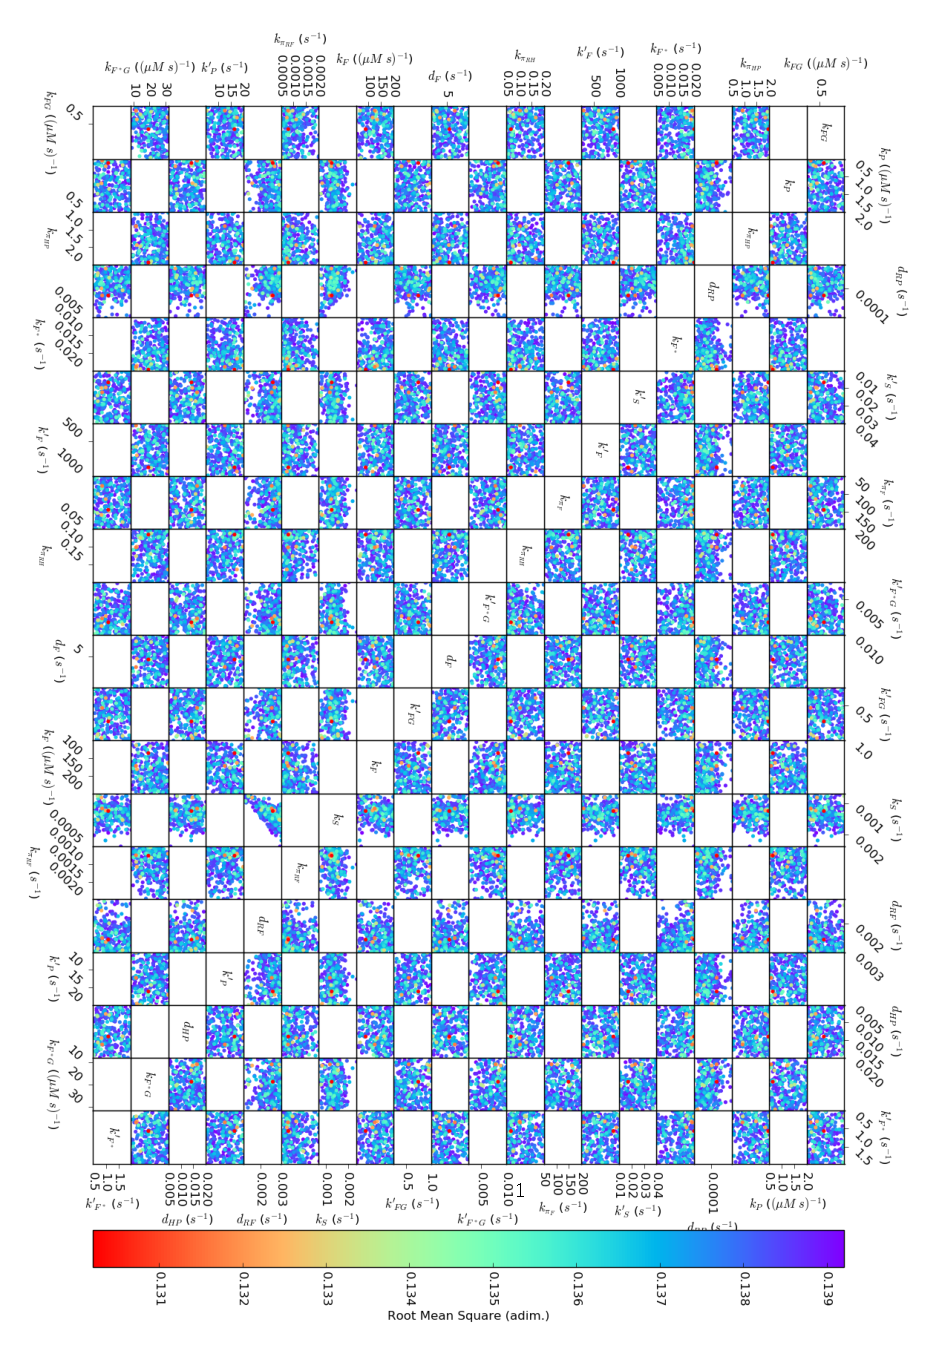
\includegraphics[width=0.88\textwidth]{Figure5_SupMat.pdf}
\caption{\small{\textbf{Projection w.r.t.~each couple of parameters of the MC scan of the parameter space.} Colors show the RMS for the same points of Fig.~\ref{Figure2label}~C, to investigate the presence of correlations among them.}
}
\label{Figure5label}
\end{figure*}


{Interestingly}, the parameter set which provides the best RMS among this randomly 
generated {sets (i.e. the isolated point at the very bottom of each panel in Fig.~\ref{Figure2label}~C), 
fails to reproduce key features that the real system has shown in the experiments, when used 
to simulate other situations, in particular the double heat shock experiment shown in Fig.~\ref{Figure3label}~C.
For instance the capability of showing a second HSR of the same amplitude as the first only when the duration between the
two consecutive HSs lasts for at least 5h cannot be reproduced.
Furthermore, other parameter sets providing a low RMS in the MC approach were exhibiting oscillations in the concentrations 
of $mR_{F}$ and $mR_{HP}$, which have not been observed in experiments. 
In principle, the double heat shock experiment data could also be included in the calibration procedure, but this would require some 
rather arbitrary assumptions as described in Supplementary Material~\ref{sectionRMS2HS}, and thus we discarded that approach.}
%turns out to be not a viable one, because if used to run the simulations of other situations as for instance the double HS, it provides to the model a behaviour qualitatively different from what is observed in the experiments.

{These observations lead us to conclude that many very different configurations distributed in the whole parameter space would 
result in a small RMS, but fail to reproduce key features. Since the fiducial parameter set reproduces all desired features and, moreover,
results in an only slightly higher RMS than the lowest obtained by the random sampling approach, we chose a gradient search for a
local optimization of the manually tuned fiducial parameter set.}


On the other hand, if we consider small variations of one parameter at a time, we observe smooth variations in the RMS values, indicating that the RMS is roughly parabolic for perturbations of each one of the majority of the parameters around the corresponding fiducial value, and that the fiducial value often lies {already} close to the minimum. 

In Fig.~\ref{Figure10label} we show that the final parameter values (indicated by yellow starts), obtained with the local optimization (gradient search, see next section), lie indeed around the minimum of an RMS landscape which is roughly parabolic w.r.t. individual perturbations of (the great majority of) the parameters. {This figure shows how much the RMS decays for small changes in any of the 20 rate constants considered in our fitting procedure and listed in Table~\ref{TabKs}. We have here considered small variations of one parameter at a time, adding or subtracting up to $80\%$ of its final value, for each parameter. For a parameter with fiducial value e.g. $100$ $s^{-1}$, this means considering the range from $20$ $s^{-1}$ to $180$ $s^{-1}$, which contributes to the asymmetry in the majority of the sub-panels of Fig.~\ref{Figure10label}, where the RMS appears to grow more when lowering the corresponding rate constant. We can also remark how the fiducial parameter values, indicated by a red vertical line, are indeed already close to the values minimizing the RMS for each parameter.} 

We clearly see that for similar perturbations different parameters produce drastically different changes in the RMS. While over the range of perturbations considered some parameters induce changes in the RMS spanning only the range from $0.14$ to $0.16$, some other parameters lead to increases of the RMS up to about $0.40$. This analysis provides thus an idea of how important each parameter is to the overall quality of the model fit and it might offer some motivation for future experimental work, by suggesting which parameters it would be most useful to measure empirically, where possible. %We finally notice that by changing only one parameter at a time the RMS does not decrease below $0.140$.
% (as shown in the example of Fig.~\ref{figure3}). 


\begin{figure*}[h!]
\centering
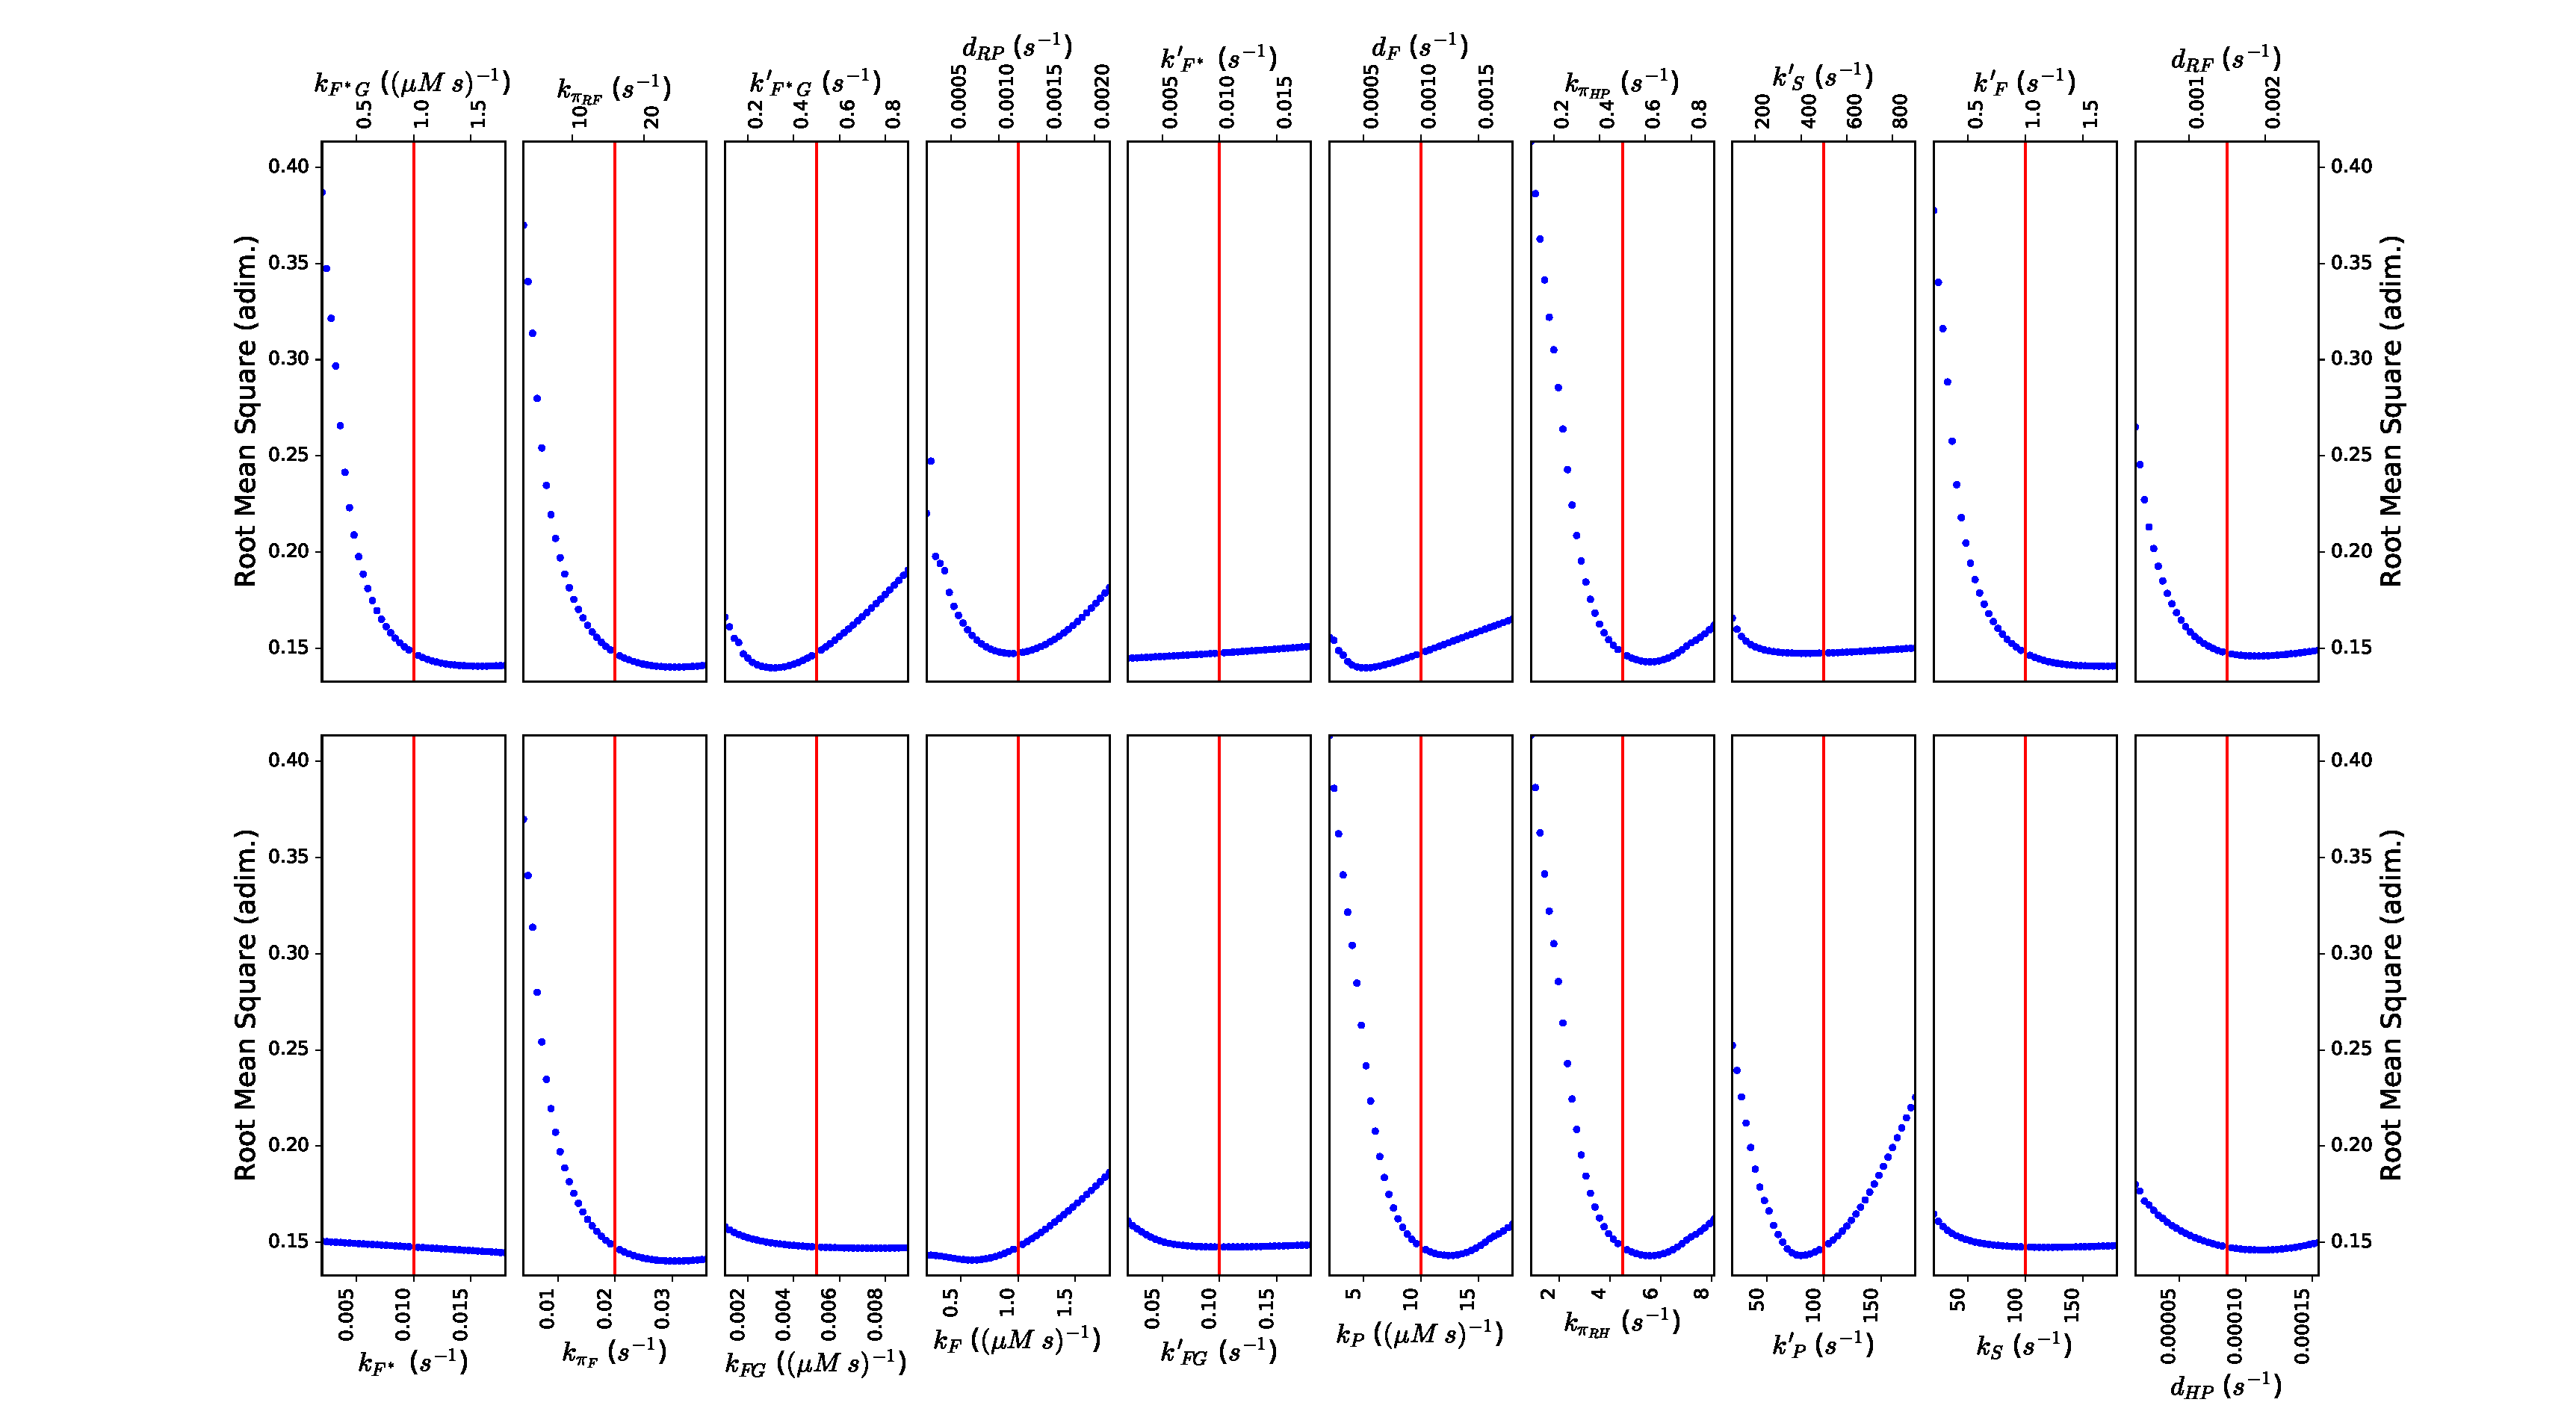
\includegraphics[width=\textwidth]{Figure10_SupMat.pdf}
\caption{\small{{\textbf{Sensitivity analysis: effect on the RMS of small perturbations in each parameter.} Each sub-panel shows the changes in the RMS occurring for small perturbations of one parameter at a time. These perturbations are performed around the final parameter values (indicated in the figure by yellow stars) obtained with the local optimization. The vertical red line in each sub-panel indicates the fiducial value of the corresponding parameter, i.e. the starting point of the two alternative calibration approaches used, the MC and the gradient search finally employed. For each parameter separately, perturbations are performed by adding or subtracting up to $80\%$ of its final value to itself.}}}
\label{Figure10label}
\end{figure*}
 

%\begin{figure}
%\centering
%\includegraphics[width=\columnwidth]{figure3.pdf}
%\caption{REMOVE? Example of figure showing RMS versus one of the model's parameters, when we consider variations %only in one of the parameters at a time. The points aligned along the vertical line in the center of the figure %correspond to variations in one of the other parameters, and are showed for comparison. We repeated this analysis %for the 20 parameters of the model.}
%\label{figure3}
%\end{figure}

Thus, after having performed a global random scan of the parameter space to gain a better understanding of how the RMS {behaves} in it, we decided to determine the final parameter set by employing {instead} a local optimization method, namely a gradient search starting from the fiducial parameter set. 
This provides a parameter set allowing a better fit to the data used to compute the RMS, while not moving too far away from our already {plausibly} behaving fiducial set. 
%It is important here to recall the generality of the model's description of the HSR, and the lack of measurements on the parameters involved. Thus the goal of the model is, given an input (the temperature as function of time), to simulate a plausible output (the behaviour of the concentrations as functions of time), and not to determine the "internal" parameters involved (the rate constants). 

%\begin{figure*}
%\centering % angle=90,
%\hspace*{-1.6cm}\includegraphics[width=1.3\textwidth, height=0.55\textheight]{ScatterPlot400.pdf}
%\caption{2-dimensional projection w.r.t. each couple of parameters of the Monte Carlo scan of the parameter space, showing RMS (colors) for the same points of Fig.~\ref{Figure1}, to investigate the presence/absence of correlations among them.
%}
%\label{{Figure5label}}
%\end{figure*}





\subsection{Local optimization using a gradient search to fit the parameters' values to the data}

%(FIXME: update the values of the RMSs etc. in this section to the most recent run) 
As discussed above, the fiducial set of parameters allows already to obtain a value of the RMS {which is close to the lower value of the RMS obtained considering the random parameter sets. In fact we} explored the parameter space with the MC analysis and we concluded that the RMS can be improved only marginally w.r.t. the value corresponding to this set. %the fiducial parameter set, and that very diverse sets of parameters can achieve this goal, meaning that different regions of the parameter space can provide a good RMS and thus can be used for our model. 
Having shown that no region of the parameter space is preferred by the RMS, we opted for a local optimization procedure, thus performing a gradient search starting from the point represented by the fiducial set of parameters, 
%We thus decide to apply an optimization procedure to improve the fit of the model to the data, but we do so with a local optimization, which we consider sufficient for the purposes of our model.
%We do so by implementing a gradient search, and in particular using 
employing the steepest descent method. 

This means that we start from a point $\vec{x}_0$ in the parameter space represented by the fiducial values for the 20 rate constants employed in our model (see Table~\ref{TabKs}). We compute the corresponding value of the root mean square $RMS\left(\vec{x}_0\right)$. We then compute numerically the gradient of the RMS at that point $\vec{\nabla}RMS\left(\vec{x}_0\right)$ (by approximating partial derivatives using the symmetric difference quotient). 

%\begin{figure}
%\centering
%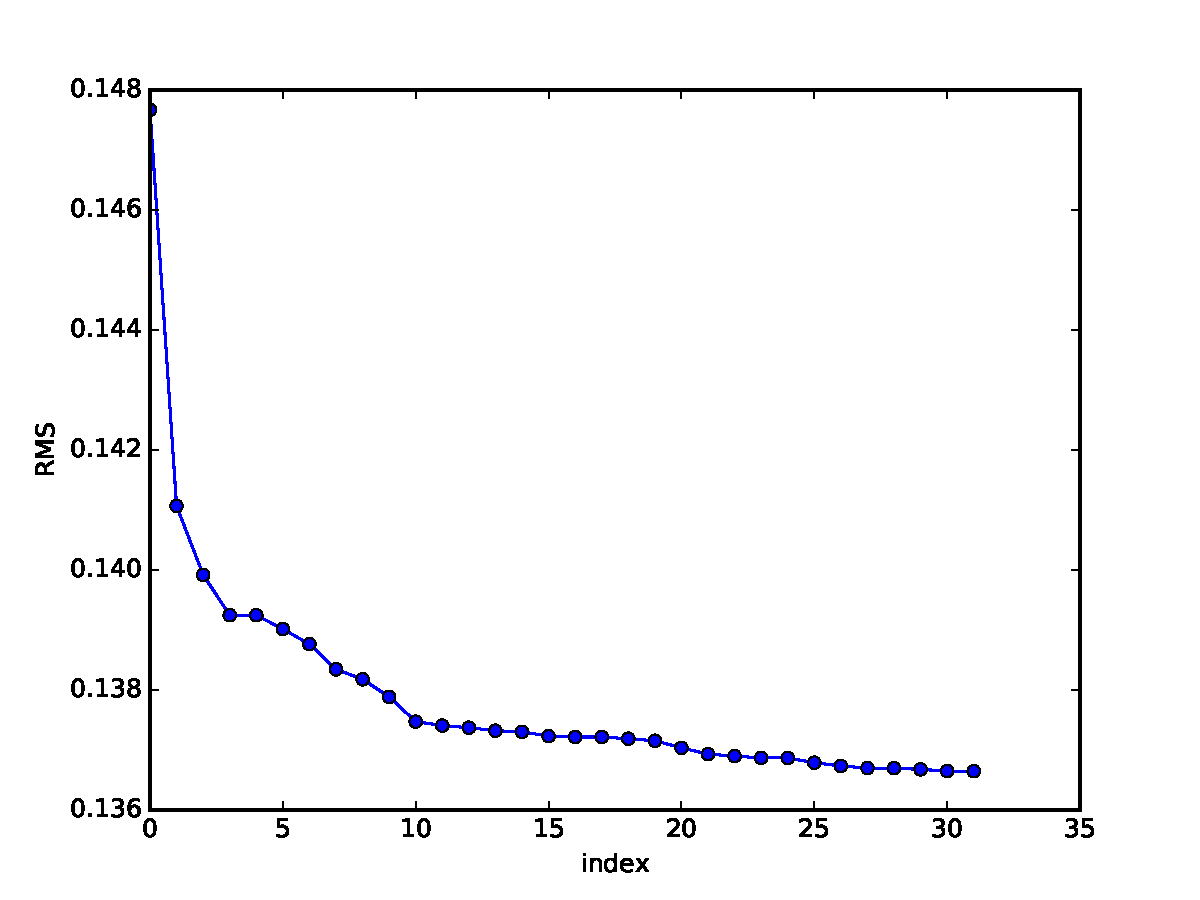
\includegraphics[width=\columnwidth]{GradientSearch_RMS.pdf}
%\caption{RMS decrease for subsequent iterations of the gradient search algorithm.}
%\label{GradientSearch_RMS}
%\end{figure}

We then proceed along the direction opposite to the gradient towards a new point \mbox{$\vec{x}_{n+1} = \vec{x}_{n} - \gamma\vec{\nabla}RMS\left(\vec{x}_n\right)$} in the parameter space which provides a smaller value of the RMS. We do so iteratively until a termination criterion described below is satisfied, and label the iteration number by $n$.
At each iteration, we need to decide which is the length of the step $\gamma$ that we want to use in the direction opposite to the gradient. To do so, we implement a line search with the aim to loosely minimize the function $f\left(\gamma\right) \doteq RMS\left(\vec{x}_{n} - \gamma\vec{\nabla}RMS\left(\vec{x}_n\right)\right)$ w.r.t. $\gamma$, i.e. along the direction opposite to the gradient. This means finding the value of $\gamma$ which minimizes the function $f\left(\gamma\right)$. We do so numerically employing a modification of the bisection rule based on the Golden ratio to save computation time. 

Since the orders of magnitude of the parameters are very different, we expect the isosurfaces of the function $RMS\left(\vec{x}\right)$ to be far away from being spherical. This would lead to a very slow convergence of the method, because the gradient at each step would hardly point roughly toward the minimum. We thus employed also a preconditioning of the function that we want to minimize, i.e. the RMS. This means that we applied the numerical procedure of minimization not to the actual $RMS\left(\vec{x}\right)$, but to a function $RMS'\left(\vec{x}'\right)$ which we obtain by transforming $RMS\left(\vec{x}\right)$ via a rescaling of all the parameters using their fiducial values. In this way all the parameters are of order of magnitude 1, which is more suitable for the application of the described numeric algorithm. Once the minimization has been performed, we applied the inverse transformation to re-obtain the parameters in their original form.

The termination criterion we employed {forces} the algorithm to stop when the average RMS decrease over the last ten iterations is lower then a threshold value. This criterion is of course somewhat arbitrary, but we have selected it by empirically verifying that it allows a better fit to the control data (a lower RMS), avoiding an over-fitting which would lead to model behaviour too far away from the behaviour expected w.r.t. other situations as e.g. the double HS. %as can be seen from Fig.~\ref{GradientSearch_RMS} and Fig.~\ref{GradientSearch_kFsp}.
The algorithm stopped after 31 iterations (Fig.~\ref{Figure2label}~D) and returned the set of parameters listed in the second column of Table~\ref{TabKs} as final values. The corresponding value of the RMS w.r.t. the controls of the feeding experiments is $0.137$.  We have employed this set of parameters to perform all the simulations shown in this work ({apart} from the calibration runs).


%\begin{figure}
%\centering
%\includegraphics[width=\columnwidth]{GradientSearch_kFsp.pdf}
%\caption{Values of one of the parameters for subsequent iterations of the gradient search algorithm.}
%\label{GradientSearch_kFsp}
%\end{figure}


\subsection{Exploring the possibility of an alternative RMS}
\label{sectionRMS2HS}

As a final test we defined, similarly to what we have done above, a RMS distance between the model simulations and the experimental data from the double HS experiment of Schroda et al. \cite{Schroda2000}. Defining such an RMS is much more arbitrary than defining the RMS w.r.t. the controls of the feeding experiments, because of the previously mentioned hypothesis on the proportionality between the enzyme concentration and its activity. %This is ways more arbitrary and approximate, given that we would have to compute this RMS combining data about the activity of the ARS enzyme with model predictions about the concentration of this enzyme. Moreover, it would then become necessary to combine the RMS w.r.t. the controls of the feeding experiments, and 
We do not combine the two RMSs, as this would require to attribute to the two a weight which would be highly arbitrary. 

For these reasons we only compute this second RMS a posteriori as a check, for the best {(i.e. here those with $RMS < 0.149$ w.r.t. the data of the feeding experiments)} among the random parameters sets selected above, and show the distribution of the values of the two different RMS in Fig.~\ref{Figure6label} of the Supplementary Material. This shows that minimizing both at the same time cannot be obtained, and one needs to find a trade-off between the two. The values of the RMS w.r.t. double HS run between $0.11$ and $0.55$ (not all visible in the figure, which is magnified). We can a posteriori compute this RMS for the fiducial parameter set, finding $0.170$, and for the final parameter set, obtaining $0.168$.

Finally, we verified that in the gradient search performed in the previous section, if we employ the sum of the two RMS instead of the RMS w.r.t. to feedings only, we can improve the fit to the double HS data, but at the cost of having non-realistic behaviours in the model consisting of big oscillations in the concentrations after onset of HS (and of introducing an arbitrary weight between the two RMSs). We eventually decided to employ for the calibration only the RMS w.r.t. the feeding data.

%\begin{figure}
%\centering
%\includegraphics[width=\columnwidth]{{Figure6label}.pdf}
%\caption{RMS w.r.t. the double HS data of Fig. \ref{ARS2} versus RMS w.r.t. the controls of the feeding experiments of Fig. \ref{2D}, magnifying the region where the points with lowest values of the RMSs lie. %This shows that minimizing both at the same time cannot be obtained, and one needs to find a trade-off between the two. As discussed in the text the point with lowest RMS w.r.t. feeding experiments exibhit, despite the low value of the second RMS, a behaviour that contrast whit that observed on the double HS experiments, and thus we do not consider it as a viable set for our model.
%}
%\label{{Figure6label}}
%\end{figure}



%\subsection{The model reproduces the qualitative behaviour observed in the experiments}

%We have compared the results of our simulations to the corresponding experimental data, those of the second group. These are the double heat shock experiments performed in \cite{Schroda2000} and shown in Fig.~\ref{Figure7label} and the feeding with Staurosporine and Radicicol performed in \cite{Schmollinger2013} and shown in Fig.~\ref{Figure3label}~(A-B). Additional comparison with data on the expression of the HP protein collected in \cite{Muehlhaus2011} are shown in Fig.~\ref{Figure3label}~D. 

%The figures mentioned above show the corresponding results of the simulations performed with our model using the final parameter set determined as described in the previous section. 
%The experimental set-ups, the salient features of each experiment and the way to use our model to simulate these experiments have been widely described in Sections \ref{SecFeeding} and \ref{Sec2HS}.
%As we can see from the figures, the model reproduces well the qualitative and the (relative) quantitative behaviour of these experimental data.


\begin{figure}
\centering
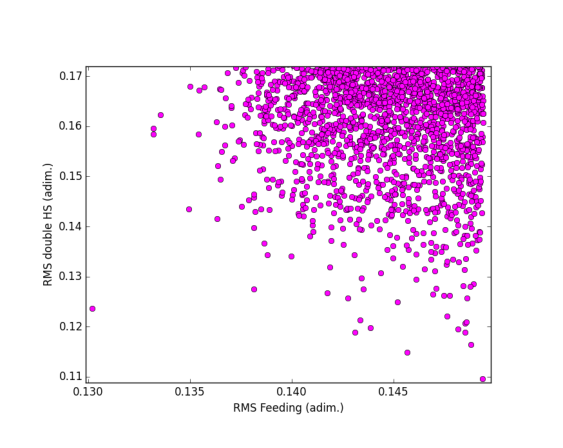
\includegraphics[width=\columnwidth]{Figure6_SupMat.pdf}
\caption{\small{\textbf{RMS w.r.t. the double HS data of Fig.~\ref{Figure3label}~C versus RMS w.r.t. the controls of the feeding experiments of Fig.~\ref{Figure2label}~(A-B).} The figure shows a magnification of the region where the points with lowest values of the RMSs lie.  %This shows that minimizing both at the same time cannot be obtained, and one needs to find a trade-off between the two. As discussed in the text the point with lowest RMS w.r.t. feeding experiments exibhit, despite the low value of the second RMS, a behaviour that contrast whit that observed on the double HS experiments, and thus we do not consider it as a viable set for our model.
}}
\label{Figure6label}
\end{figure}


%\subsection{{An alternative possible approach to the calibration of this model}}

%{The MC sampling from the joint prior parameter distribution which we performed here just provided us a hint on the structure of the 20-dimensional parameter space, without exploring it extensively. The local optimization method which we used instead, the gradient search, neither leads to an extensive exploration of the parameter space, nor to identify a unique parameter set. As already underlined, our goal was not to uniquely identify the best parameter set according to the RMS (only based on a rather small dataset), or to fully characterize the correlations among parameters. Our goal was instead to identify one (among many) viable parameter set, to verify that the model structure (signalling network of Fig.~\ref{Figure1label}~A, ODEs and rate laws of Supplementary Material Table~\ref{TabVars} and Table~\ref{TabNUs}) could indeed reproduce the behavior observed in several experimental data sets (Fig.~\ref{Figure3label}).
%To extensively explore the 20-dimensional parameter space, to identify a most suitable parameter set, and to perform an in-depth study of parameters correlations, more elaborate methods could be applied. For instance, we could define a Likelihood function incorporating the joint prior probability distribution which we assumed for the model parameters, together with the probability distribution of observing the measured data provided the values of a given parameter set. This last could be based on the root mean square deviation of the observed values from those obtained from the model for any given parameter set, e.g. assuming Gaussian measurement noise. While usually it is not easy or not even possible to compute the resulting Likelihood function, this could be overcome by applying a Markov chain Monte Carlo (MCMC) method, e.g. the well known Metropolis-Hastings algorithm. This would allow to obtain an estimate of the posterior probability distribution for the model parameters, and ultimately to identify the best estimate of the parameters and the corresponding variance providing an error on their estimate. Correlations among model parameters could have been studied by computing the corresponding covariance matrix. We have left such an approach for future potential developments since, as explained above, we consider it beyond the scope of this work.}




\clearpage

\section{Supplementary Material: double heat shock characterization}

We present here some additional simulations which illustrate extensively the features of the response to a double HS, and next we explain how we have extended our model to simulate the double HS experiments performed in Schroda et al. \cite{Schroda2000}.




\subsection{Simulating the double HS experiments to investigate their main features}
\label{Sec2HSsimulations}

Fig.~\ref{Figure7label} shows four {groups} of panels illustrating how the HSR dynamics changes when we simulate a generic double HS experiment, providing to the system two HSs separated by $30$ min (A-F), $2$ h (G-L), $3$ h $30$ min (M-R) or $5$ h (S-X). We provide a sudden variation of the temperature between 25°C and 42°C. {In each simulation, the first HS lasts $120$ minutes and starts at $t=40$ minutes, while the second HS lasts until the end of the simulation.}

As we can see from Fig.~\ref{Figure7label}, when the second HS occurs only $30$ min after the first, the system shows almost no response to the second. This is due to the fact that during the first HS, thanks to gene activation (panel D) and subsequent production of mRNA for the HSF (panel E), the quantity of HSF available to the system increases (panel C). When the second HS occurs, $30$ min after the end of the first, the HSF available to the cell is already enough and no activation of the SK takes place (panel B). When the second HS occurs a lot of HSP is still available in the system (panel F) and thus the level of $P^\#$ does not increase (panel A). When the second HS occurs $2$ h after the first, there is a small HSR during the second, visible at the level of SK (panel H) and of mRNAs (panel K). This because even if a lot of HSP is still available (panel L), the HSF concentration is very low (panel I) and then a moderate HSR is necessary to allow the system to quickly refold unfolded proteins. 
The HSR corresponding to a second HS occurring at $3$ h $30$ min after the first is similar, but enhanced. 
When the second HS occurs $5$ h or more after the first, the concentration of HSP is approaching the level it had before the HS (panel X), all the other quantities are back to the original values, and an almost full HSR takes place during the second HS (panels T-W). 

It is very interesting to remark that, while the concentrations of all the species {after the end of the first HS go back to the values that they had before the first HS quite fast, the HSP does not (panel X). This allows to have only a much smaller amount of unfolded protein $P^\#$ during the second HS w.r.t. the amount during the first HS.} This can be seen in panels A, G, M and S, where the concentration of degenerated proteins $P^\#$ increases by a considerable amount during the first HS, while considerably less during the second even when this is occurring many hours after the first. % has the role of preparing the system for a subsequent occurrence of the same stressing situation (HS) already encountered in the past, thus representing a sort of molecular "memory" of the Chlamydomonas cells. 
The behaviour we observe in our simulations likely indicates that the production of HSF which follows a first HSR and the accumulation and slow degradation of HSP has the role of preparing the system for a subsequent occurrence of the same stressing situation (HS) already encountered in the past, thus representing a transient molecular memory. This observed behaviour is consistent with the claim of Schroda et al. \cite{Schroda2000} that \emph{Chlamydomonas reinhardtii} needs around $5$ h {after a first HS to recover and exhibit a HSR during which the increase in $HSP$ concentration has the same amount as during the first HSR.} %We have seen in the main text a direct comparison of simulations performed with our model and data from \cite{Schroda2000}, and in the next section we provide additional details on how we have extended our model to perform such simulations.

%\begin{figure*}
%\minipage{0.50\textwidth}
%  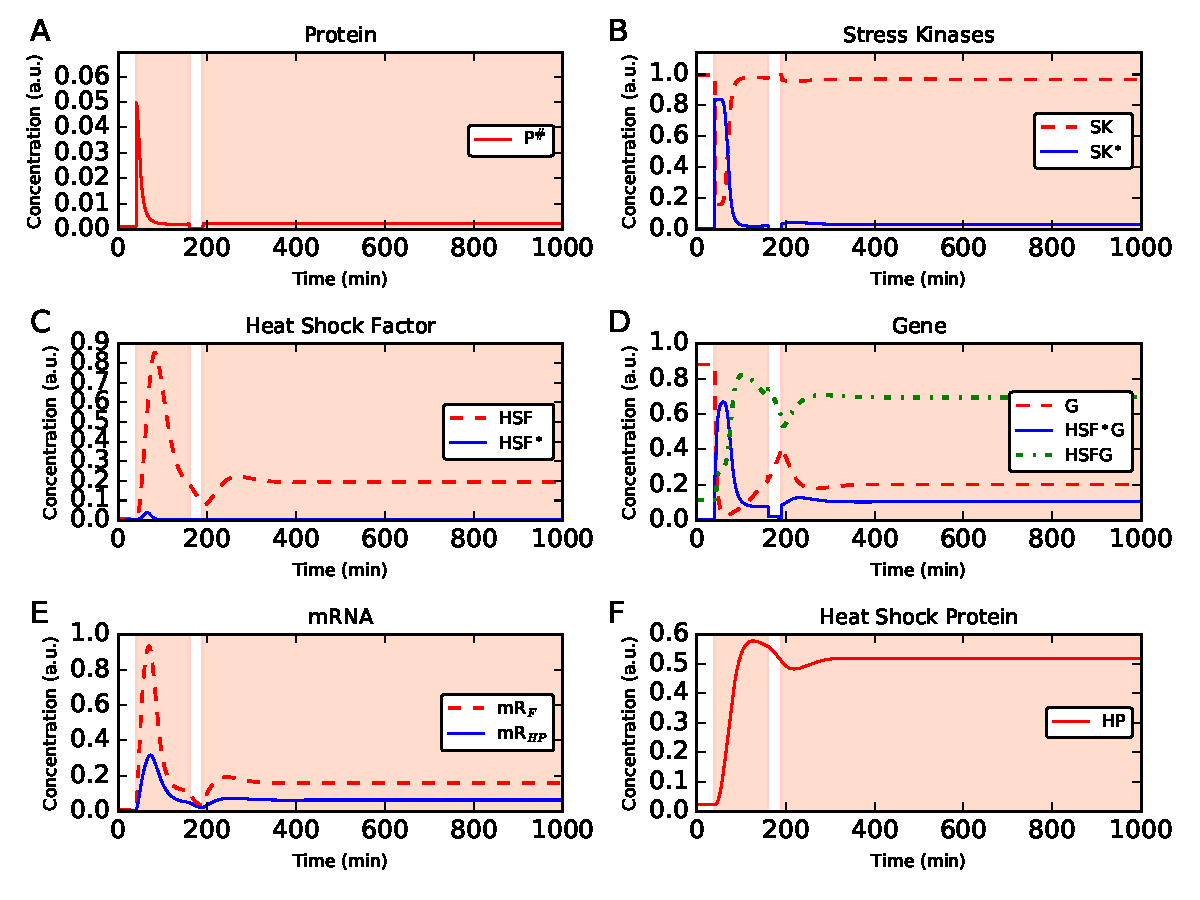
\includegraphics[width=\textwidth, height=0.35\textheight]{HeatShockResponse_SimulationDoubleHeat30min.pdf}
%  \caption*{\small{Second heat shock after 30 minutes.}}
%\endminipage\hfill
%\minipage{0.50\textwidth}
%  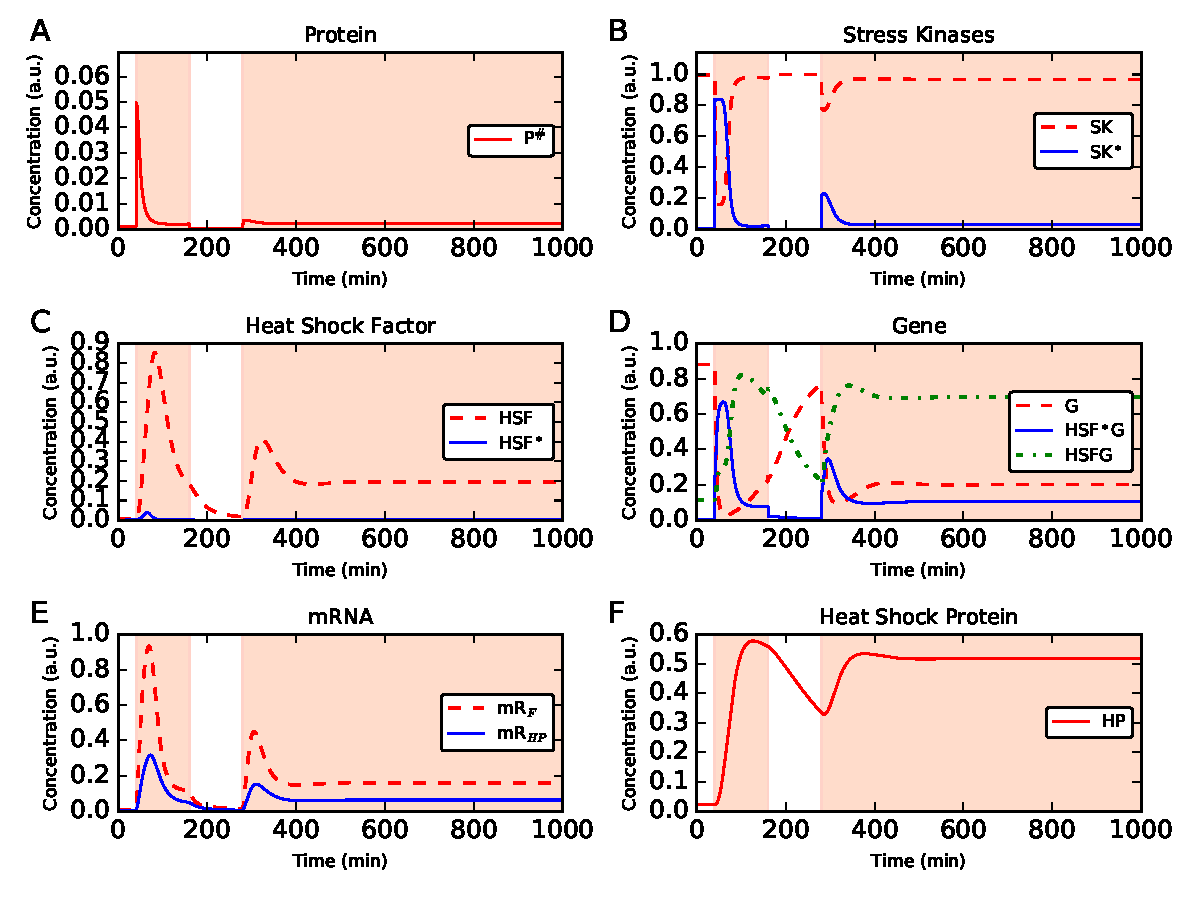
\includegraphics[width=\textwidth, height=0.35\textheight]{HeatShockResponse_SimulationDoubleHeat2h.pdf}
%  \caption*{\small{Second heat shock after 2 hours.}}
%\endminipage\hfill
%\minipage{0.50\textwidth}
%  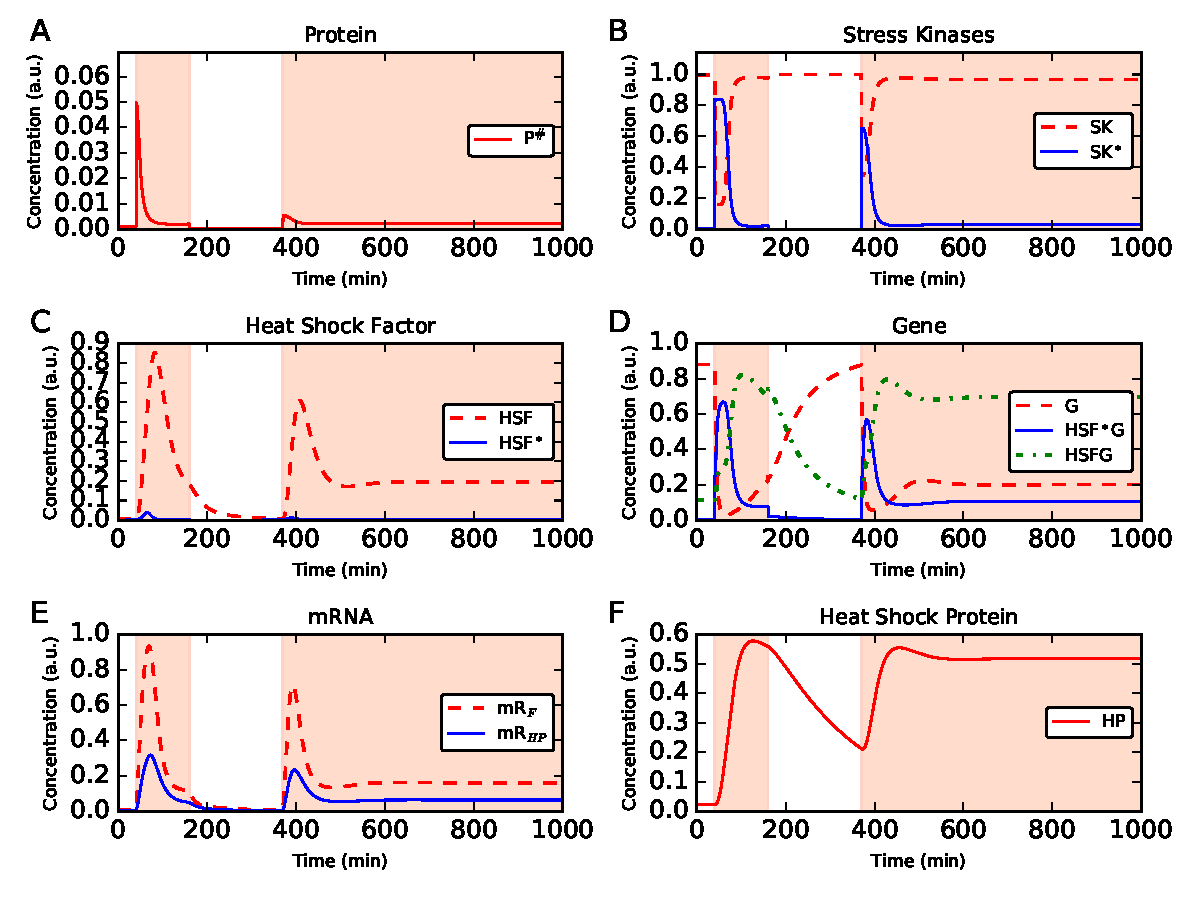
\includegraphics[width=\textwidth, height=0.35\textheight]{HeatShockResponse_SimulationDoubleHeat3h30min.pdf}
%  \caption*{\small{Second heat shock after 3 hours and 30 minutes.}}
%\endminipage\hfill
%\minipage{0.50\textwidth}
%  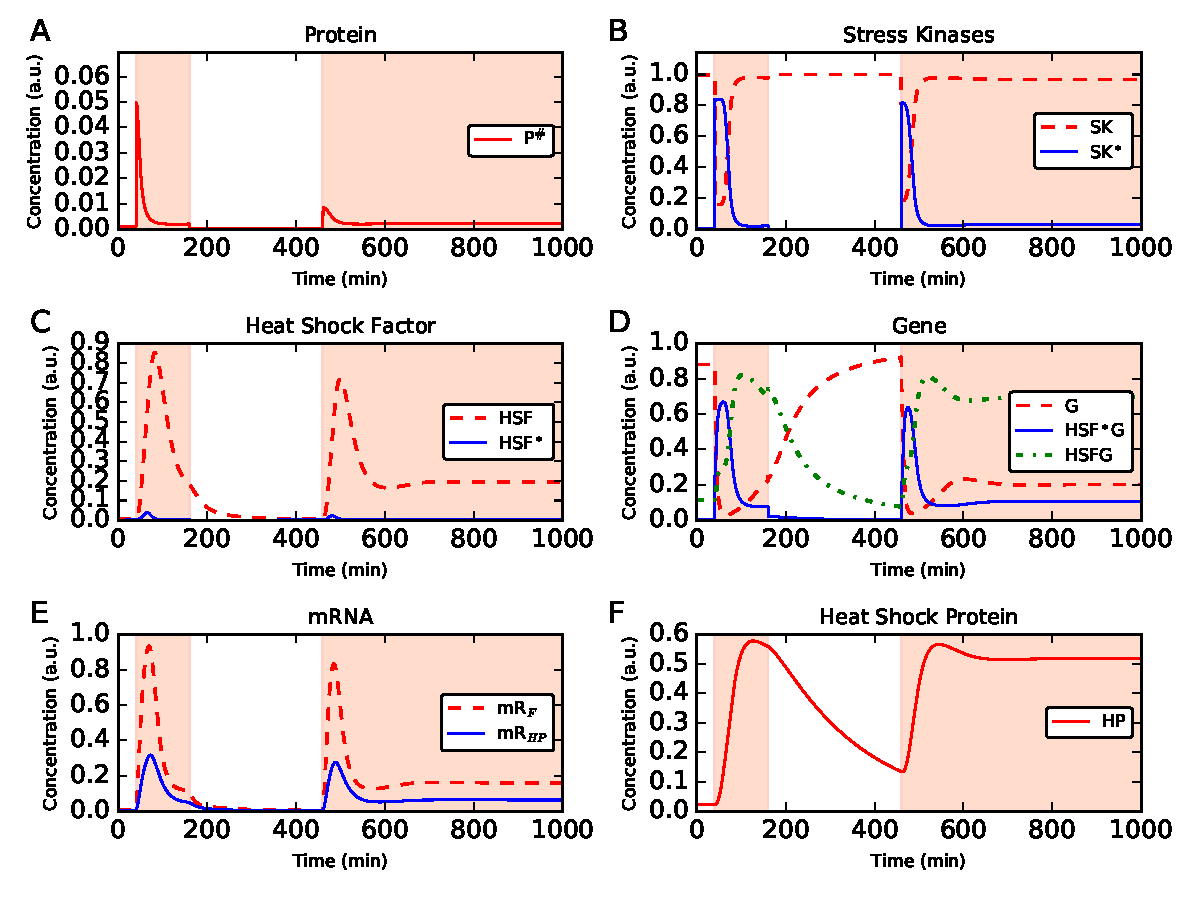
\includegraphics[width=\textwidth, height=0.35\textheight]{HeatShockResponse_SimulationDoubleHeat5h.pdf}
%  \caption*{\small{Second heat shock after 5 hours.}}
%\endminipage\hfill
%\caption{\small{Simulation of a generic double heat shock experiment. The second heat shock is provided respectively after $30$ min, $2$ h, $3.5$ h and $5$ h. We can appreciate how the dynamics changes at the level of each species. Particularly relevant is the fact that a full response to the second HS is possible only after about $5$ h, as clearly shown by e.g. the SK$^*$, HSF$^*$ and mRNAs curves.}}
%  \label{Figure7label}
%\end{figure*}






\subsection{Extending the model to simulate the experiments on the double HS}
\label{SecARSSM}

To perform the simulation reproducing the data of Schroda et al. \cite{Schroda2000} (Fig.~\ref{Figure3label}~C of the main text), we extended our model including few new variables and equations. 
We included the production of ARS enzyme by adding two new variables and four new reactions. 
These are listed in Table~\ref{TabARS}, together with the corresponding ODEs and parameters values.
The two variables represent the concentrations of the mRNA coding for the ARS enzyme (due to fusion of the ARS gene on the HSP70A promoter), and that of the ARS enzyme.
The four new reactions that we added describe the production of mRNA coding for the ARS enzyme from G*HSF, the translation of ARS mRNA into ARS enzyme (i.e. production of ARS), a very slow degradation of the ARS enzyme and degradation of ARS mRNA. 
%\begin{figure}
%\centering
%\includegraphics[width=\columnwidth]{HeatShockARSExp_SimulationARSexperiment.pdf}
%\caption{Comparison of simulations (upper panels) with data from \cite{Schroda2000} (lower panels) on single heat shock experiment to verify that the extension of our model allows to reproduce the behaviour observed therein.}
%\label{ARS1}
%\end{figure}
We selected the values of the free parameters in order to match the observations. 
%In we studied the behaviour of the added part of the system and we compare it with experimental data, verifying that the qualitative behaviour is similar.
%Applying an HS of 1h by increasing the temperature from 23°C to 40°C we have an increase of the concentration of the mRNA for the ARS enzyme due to the increase of HSF*G in our model, which reaches a peek and then drops (panel A). We also have an increase of the concentration of the ARS enzyme delayed w.r.t. that of the mRNA (due to the additional time necessary for protein synthesis), and which has a much slower attenuation (panel B) so that it takes ways longer to the ARS concentration to drop that to the mRNA concentration. We can compare the predicted concentration of mRNA with the measured one (panel C, data from \cite{Schroda2000}, and the predicted concentration of ARS enzyme with the measured ARS activity (panel D, data from \cite{Schroda2000}, Fig.~6~b). 
The comparison in Fig.~\ref{Figure3label}~C requires the simplifying, but  reasonable, additional assumption that the activity of the ARS enzyme is roughly directly proportional to its concentration. 
%Given the simplicity of the extension that we used to include this into our model, and the rough estimation of the involved parameters, 
Despite these simplifications, the qualitative agreement between \mbox{simulation and data is remarkable.} 
%to be sufficient for our purposes of reproducing the data described below.  
%Let us remark that, as occurred also in the comparison with the time course data, in the model both ARS and mRNAARS grows faster then the data (on the other hand the model is not faster when compared to the data from Shmollingen 2013, from which the model has been derived, on which it has been calibrated).

%\clearpage

\begin{figure*}%[h]
\centering
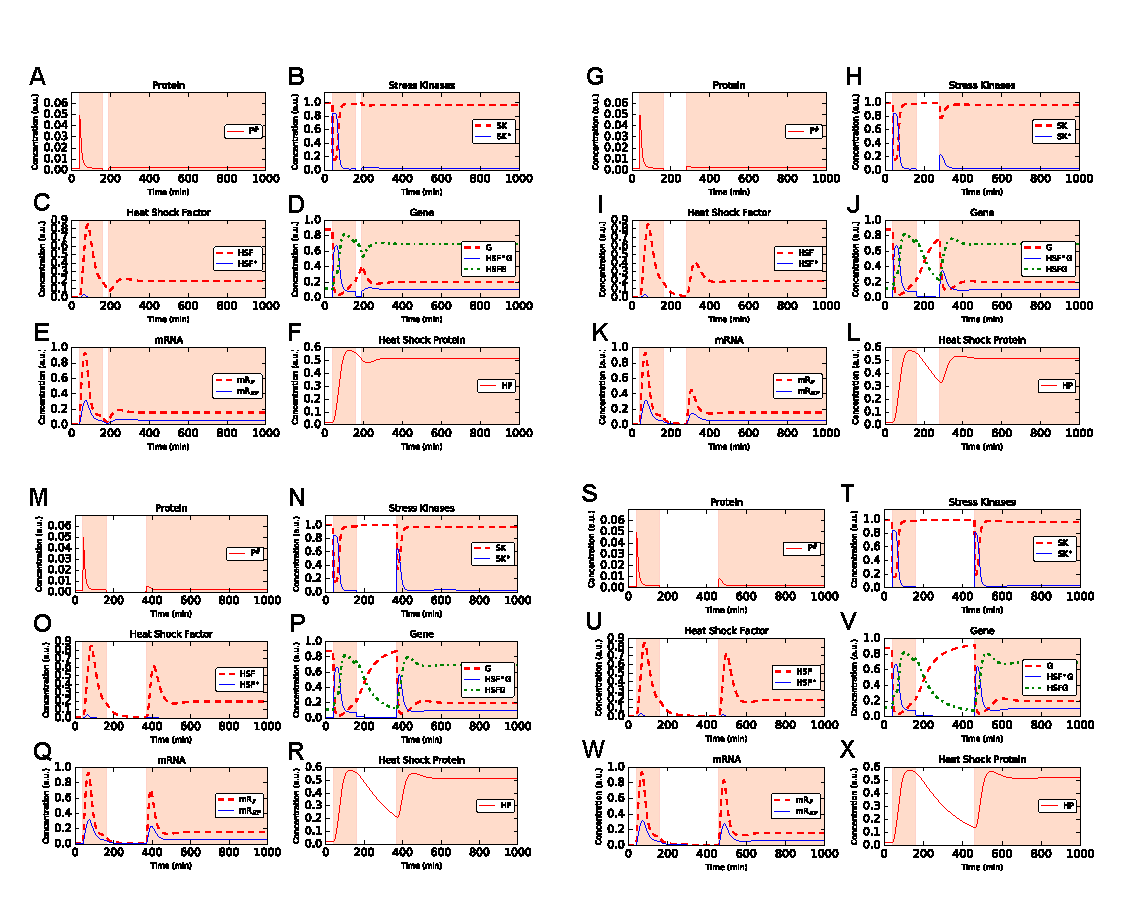
\includegraphics[width=\textwidth]{Figure7_SupMat.pdf}
\caption{\small{\textbf{Simulation of a generic double heat shock experiment.} The second heat shock is provided respectively after $30$ min \textbf{(A-F)}, $2$ h \textbf{(G-L)}, $3.5$ h \textbf{(M-R)} and $5$ h \textbf{(S-X)}. We can appreciate how the dynamics changes at the level of each species. Particularly relevant is the fact that a full response to the second HS is possible only after about $5$ h, as clearly shown by e.g. the SK$^*$, HSF$^*$ and mRNAs curves.}
}
\label{Figure7label}
\end{figure*}

\bgroup
\def\arraystretch{1.5}%  1 is the default
\begin{table*}%[h]
\[\begin{array}{ll}
\toprule
  \text{\textbf{Variable}}                     & \text{\textbf{Concentration of}} \\
\midrule
  \left[mR_{ARS}\right]                        & \text{mRNA for ARS enzyme}          \\
  \left[ARS\right]                             & \text{ARS enzyme}                \\
\midrule
  \text{\textbf{ODE}}                         & \text{ }                         \\
\midrule
 \frac{d\left[mR_{ARS}\right]}{dt} = \pi_{RARS} - \eta_{RARS} & \text{ }          \\
 \frac{d\left[ARS\right]}{dt} = \pi_{ARS} - \eta_{ARS} & \text{ }                  \\
 \midrule
  \text{\textbf{Rate law}}                     & \text{\textbf{Reaction}}         \\
\midrule
  \pi_{RARS}  = k_{\pi_{RARS}} \cdot [HSF^*G]  & HSF^*G: HSF^*G + mR_{ARS}            \\
  \pi_{ARS}   = k_{\pi_{ARS}} \cdot [mR_{ARS}] & mR_{ARS}: mR_{ARS} + ARS           \\
  \eta_{RARS} = d_{{RARS}} \cdot [mR_{ARS}]    & mR_{ARS} \dashrightarrow         \\
  \eta_{ARS}  = d_{{ARS}} \cdot [ARS]          & ARS \dashrightarrow              \\
\midrule
 \text{\textbf{Rate constant}}                 & \text{\textbf{Value}}            \\
\midrule
    k_{\pi_{RARS}}                             & 36 \text{ s}^{-1}                \\
    k_{\pi_{ARS}}                              & 0.000125 \text{ s}^{-1}          \\
    d_{RARS}                                   & 0.0012 \text{ s}^{-1}            \\
    d_{ARS}                                    & 0.0000125 \text{ s}^{-1}         \\
\bottomrule
\end{array}\]
\caption{\textbf{Extension of the model to include ARS production.} Variables, ODEs, rate laws and rate constants used to extend the model in order to simulate the double HS experiments which measure the expression of the ARS enzyme put under the control of the HSP70A promoter, performed in Schroda et al. \cite{Schroda2000}. The parameters values above are manually selected in order to reproduce the observations.}\label{TabARS}
\end{table*}
\egroup

\clearpage





\section{Supplementary Material: steady state characterization and further applications of the model}
\label{SectionFurtherPredictions}

One of the main advantages of a mathematical model, inferred and calibrated from experiments, is that {such a model often can be used to simulate situations which are difficult to test with experiments and to compute quantities which are difficult to measure.}

Thus, in this section we employ our model to simulate {systematically} further situations that are interesting while difficult to test or not yet tested experimentally. 

With our model we thus show the ability of the system to adapt to temperatures higher than usual during heat shocks longer than three hours by shifting to a new steady state. 
We subsequently study how the steady state concentrations depend on the temperature at which the steady state is reached. 
Finally we systematically investigate how the accumulation of HSPs depends on the combination of temperature and duration of the heat shock. 





%\subsection{The HSR shows acclimation to long-term HS obtained by a shift to a new steady state}
\subsection{Prolonged heat shock}
\label{SecAcclimation}

We first investigate which response the model predicts upon exposure to a prolonged HS, and how
the system {acclimates} to persistently high temperatures.
Experimentally, the systems-wide response to long-term HS was investigated in Hemme et al.~\cite{Hemme2014},
where cells adapted to 25°C were exposed to 42°C for a period of $24$ h, followed by $8$ h at 25°C (recovery phase).

%We use our model to investigate how the system reacts to a prolonged HS (long-term HS), and how it recovers from it, and we show that it exhibits perfect adaptation to long-term HS. The long term HS on a system-wide scale is experimentally studied in \cite{Hemme2014}. Employing the same set-up used therein, we simulate this situation by increasing the temperature at $t = 0$ h from 20°C to 42°C, keeping it to the higher value for $24$ h (long term HS), and then lowering it again to 20°C for the remaining $8$ h (recovery phase).

The simulation results for this scenario, where the temperature increase was simulated at time $t=0$, are shown in Fig.~\ref{Figure8label}~(A-F).
Two distinct phases of the response can be distinguished. The first, early HS phase, lasting approximately $3$ h after applying the heat shock, 
represents the initial heat shock response, in which the internal variables respond similarly to 
the normal heat shock simulations described above (see in particular Fig.~\ref{Figure1label}~(B-G), and also the control curves in Fig.~\ref{Figure2label}~(A,B)). 
During the late HS response, lasting from $3$ to $24$ h during heat shock, the variables approximate 
a new stationary state.  
This state is characterized in particular by increased concentrations of mRNAs (panel E), and consequently 
of HSF and HSP, when compared to the corresponding concentrations before the onset of the HS. 
These elevated levels suggest an acclimation of \textit{Chlamydomonas~reinhardtii} to continuous HS conditions,
which allows to efficiently avoid the accumulation of misfolded proteins.
After reverting the conditions to normal temperatures (25°C), a recovery phase can be observed, in which
the variables relax to the original stationary state over a period of several hours.
%Thirdly, the recovery phase is characterized by the tendency of the system to go back to the state preceding the HS, but with no urgency so that after some hours still the concentration of HSP is not yet as low as before the HS. 
%Finally, while the concentration of HP during the late HS period is about $90\%$ of that corresponding to the peek during early HS, the concentration of HSF during the late period is only around $25\%$.
These results are consistent with the observations of Hemme et al. \cite{Hemme2014} focusing on HSP production (see in particular Fig.~8 therein).









\subsection{Stationary behaviour}
%\subsection{Different steady state concentrations for different temperatures allow to keep a low level of unfolded proteins}
\label{SecSteadyStateConcentrations}

%(FIXME: update this paragraph for the latest version of the figure, in particular after switching to Arrhenius law to describe the effect of temperature we need to say that now the system actually saturates when T is high enough, which is the reason for which we used this law. Add also a zoomin from 30 to 65°C of panel A.) 
The observations that the system adopts a new stable stationary state when continuously exposed to elevated temperatures
raises the question how this long-term response depends on the rate of protein denaturing. 
The steady state concentrations depend on temperature only via the speed of the reaction $P \rightarrow P^\#$, which itself depends on the temperature, and on other quantities, as described by the corresponding equation in Table~\ref{TabNUs} of the Supplementary Material based on the Arrhenius law. We now study how the steady state concentrations depend on the temperature at which the steady state is reached.

%\begin{figure}
%\centering
%\includegraphics[width=1.0\columnwidth]{UnfoldingRate.pdf}
%\caption{{\color{violet} SM: May be let's simplify the figure, only one curve (the blue)? ...and use on the vertical axes the real k of the model and remove 100/k ?} Higher temperatures (horizontal axis) correspond to higher unfolding rates (verical axes) following the Hill kinetics behaviour described by the curve with $T_0=36$°C and $n=5$, used in the model. The verical axes reports the values of the rate $\nu_P'$ divided by the concentration $\left[P\right]$, computed for a typical rate constant of $k_P'=100$ s$^{-1}$. The figure illustrates also the effects of variating the values of $n$ and $T_0$. We see that using a Michaelis-Menten behaviour ($n=1$) instead of a Hill kinetics would have not allowed to have the sigmoidal shape that well describes the presence of a thrashold temperature for the activation of the HSR.}
%\label{UnfoldingRate}
%\end{figure}

First we have intuitively verified that the system reaches a steady state by naively integrating it over very long times. %This can provide an intuitive answer to the question: "does the system reach a steady state, i.e. an equilibrium point?".
%If (for given initial conditions and parameter's values) there seems to be an equilibrium point, the set of values for the concentrations (the variables of our model) at the last instant of time of this long simulation can be used as a guess to properly find an equilibrium point. Then, we apply 
We then do it by applying the rigorous procedure which consists in looking for a root of the system 
%$\vec{f}(\vec{y})$, 
represented by the ODEs of Table~\ref{TabODEs} of the Supplementary Material, i.e. 
to find the concentrations which correspond to a steady state. 
%a point of equilibrium, which corresponds to having the right-hand side of all the ODEs equal to zero. So, for the system of ODEs $d\vec{y}/dt = \vec{f}(\vec{y})$, where $\vec{y}$ is the vector containing the variables, we want to find a point $\vec{y}_E$ such that $\vec{f}(\vec{y}_E)=d\vec{y}/dt=\vec{0}$. We numerically solve $\vec{f}(\vec{y}_E) = \vec{0}$, which means finding the zeros of the vector field $\vec{f}(\vec{y})$. 
It's best to have a good initial guess as a starting condition for the search, and the integration over a very long time performed above provides that. 
%Thus we might start from the guess for $\vec{y}$ inferred by taking the variables' values at the very high t obtained with the integration at point 0.
%Finding a root could often be done analytically, but of course it is simpler to do it numerically. 
Then, we repeat this for different values of the temperature, to see how the steady state concentrations change as a function of temperature. The result is plotted in Fig.~\ref{Figure8label}~(G-L). Let us remark that on the horizontal axes of Fig.~\ref{Figure8label}~(G-L) we have the temperature. Each point in any panel corresponds to the concentration of the corresponding species at steady state, when the steady state is reached at that particular temperature. 
We can see that the concentrations at steady state are different for different temperatures, with for instance higher values of the concentrations of mRNAs and HSP corresponding {to higher values of the temperature.} 

{On the one hand it is remarkable that, for values of the temperature not too high, the concentration of unfolded proteins at steady state is kept very low by the response of all the other species, in particular well below one percent of the total amount of proteins.} 
On the other hand, when the temperature increases considerably the HSR is {no longer} able to efficiently counteract the accumulation of degenerated proteins which accumulates at concentrations high enough to kill the cell. This accumulation is evident in Fig.~\ref{Figure8label}~G. 
%, a magnification of which is provided in Fig.~\ref{FigSteadyStadeConcentrationsZOOM}.

Finally, we have also verified 
%as described in section \ref{SecSteadyStateEquilibrium} 
that, for each of the values of the temperature that we have considered, the model exhibits a realistic stationary behaviour, i.e. the associated steady state (which is a non-equilibrium one) is stable. 
%\subsection{Verifying the stability of the steady state}
%\label{SecSteadyStateEquilibrium}
%(FIXME:FIXED shortened this considrably and moved to later section.)
%We have verified that the steady state reached by the system (which is different for every different temperature, and which is a  steady state) is stable. 
%in any case not only an equilibrium point, but also a stable one. 
To do so, firstly we computed numerically the Jacobian of the vector field associated to the ODEs system summarized in Table~\ref{TabODEs} of the Supplementary Material. 
%(i.e. the square matrix $df(\vec{y})/dy$, where $f$ and $\vec{y}$ are vectors of the same dimension). 
%Notice that they need to specify at which point you want to compute the Jacobian. 
Next, we evaluated the Jacobian of the system at the steady state 
%the point of equilibrium 
under investigation.
%, repeating for every 
%equilibrium point, each corresponding to a different value of the temperature. 
Then we computed the eigenvalues of the Jacobian to determine the stability of the steady state. 
%You then compute the eigenvalues of the Jacobian above to study the stability of the equilibrium point. Among the 12 differential equations composing the system, some are redundant due to certain quantities that are conserved. 
%Even if the system has twelve variables (listed in table \ref{TabVars}), only nine ODEs are required to model it. 
%In fact, there are three conserved quantities: $[P] + [P^\#]$, $[SK] + [SK^*]$ and $[G] + [HSFG] + [HSF^*G]$ are constants. %We can then describe the system with nine equations only (thus computing $[P]$, $[SK]$ and $[G]$ from the conservation laws, which are also listed in table \ref{TabODEs}). 
%Finally we manage to have only independent equations and 
We repeated the procedure for the steady state associated to each of the values of the temperature considered.
{For every steady state considered, all the nine eigenvalues result to have negative real part, which implies that each of the steady states considered is a stable steady state.}
%The steady state concentrations are investigated in more detail in section \ref{SecSteadyStateConcentrations}.







\subsection{{Relationship} between HS temperature and HS duration in the production of HSP}
\label{SecTradeOff}

%Attending YAS and ENCAPP lead to many interesting discussions with various people. Among them, certain lead to develope the content of this page.

%We now want to exploit the model to study systematically what is the response to various combination of HS durations and HS temperature.

The questions which we want to address in this section  
%arising from Elahe's comments, as well as from discussion with another participant (experimentalist) who was studying how Chlamy reacts to different type of stresses (and was very interested in this question) 
are the following: "is \emph{Chlamydomonas reinhardtii} more stressed for a short HS with high temperature or a long one but with a lower temperature? What is the {relationship} between the two?". A related question is "does the production of HSP {occur} only under very intense HS conditions (high temperature, long duration) or does it {occur} also for very small temperature increases or very short HSs?". 

{Moreover, since HSs induce the expression of HSP, exposing plant cells to controlled temperature increases may also represent a mean to drive the accumulation of cells proteins (HSPs, but not only) inside these cells.} This might be interesting for instance in view of enriching plants in any protein of interest (by engineering the HSPs genes and use their HS-activable promoter to induce the expression of other genes of interest). 
The question that naturally arises is then: "which is the HS set-up (duration, temperature) that maximizes the accumulation of HSPs?".

%Some researchers are interested in the possibility of enriching \emph{Chlamydomonas reinhardtii} in proteins (including HSPs) for using it for alimentary purposes, as an integrator of proteins in human diet. Independently on how this use might be viable or not, heat shock surely represents a mean to make (HSP) proteins accumulate into \emph{Chlamydomonas reinhardtii} cells, and the question that then naturally arises is: "which is the HS setup (duration, temperature) that maximizes the accumulation of HSPs?". We can summarize these in the following questions: "Is \emph{Chlamydomonas reinhardtii} more stressed for a short HS at high temperature or a long one with a lower temperature, what is the trade-off between the two?", and "does the production of HSP occurs only under very intense HS conditions (high temperature, long duration), or does it occurs also for very small temperature increases and very short HS?", "which kinds of HS setups (duration, temperature) maximize the HSP production?". 

To answer these questions we performed a systematic study of how much HSP is produced under different combinations of HS durations and HS temperatures. 
For such a study, we provided to the system a sharp increase in temperature starting from 20°C. 
Since here the goal is mainly to study under which conditions \emph{Chlamydomonas~reinhardtii} is more stressed, the response is closed only when HSP is produced and can act to refold unfolded/mis-folded proteins and the main interest in eliciting an HSR may be to induce the accumulation of HSP (or other proteins), 
we perform this study at the level of HSP production. % Moreover, different people seemed to be interested mainly in the final outcome of the HSR, i.e. the HSP, rather than the intermediate steps.

Thus we simulate the response to the different combinations of HS temperature and HS duration, and we plot the value of $\left[HP\right]$ computed right at the end of the HS period as contours in the {plane} representing HS duration versus HS temperature, and a color map is used to make the figure visually clearer. 
It is worth to point out that this time point provides a value of $\left[HP\right]$ that is not necessarily the highest one that can be obtained with an heat shock of that temperature and duration, in fact $\left[HP\right]$ grows under HS, reaches a maximum, decreases a bit and settle to a new steady state value until HS is kept on. %As seen in the plot the maximum is achieved around approximately $100$ min (for any temperature), but if the HS is kept longer, $\left[HP\right]$ is lowered a little bit. 
For short HSs, as seen previously, even if the increase in temperature is sharp, and the activation of SK follows, there is a certain inertia in the response at the level of mRNA production, and an additional delay in the HP synthesis. As a consequence if the concentration of HP is read out at the end of a short HS, it is possible that the obtained value is lower than the value one would obtain with the same HS, but waiting some more time. %after the HS to the system for taking the mRNA and expressing the corresponding HP. We thus decided to measure the $\left[HP\right]$ at the end of the HS, keeping in mind that this in certain cases is not the time point at which $\left[HP\right]$ is maximal.

Fig.~\ref{Figure8label}~M shows the concentration of HSP at the end of the HS, as a function of HS duration and HS temperature. Firstly, looking at how $\left[HP\right]$ changes for any fixed temperature, we can appreciate the same features that we already noticed in Fig. \ref{Figure1label}~(B-G). There is no response at the level of $\left[HP\right]$ for duration of less then about $10$ min, then HP rapidly goes up for longer HS, and the maximum HP concentration occurs around $80$ to $100$ min. For longer HSs $\left[HP\right]$ is somewhat lower, and does not change any more when increasing further the duration of the HS (new steady state reached, i.e. acclimation occurred).
Second, considering increasing temperatures, we can see that even a small increase of few degrees in temperature results in an increase of $\left[HP\right]$. %For short HS (smaller than $10$ min), no HSP is produced, no matter how high the temperature is. 
%3) If we look at both together, we can easily understand from the plot the trade-off between duration and Temperature, and draw conclusions as for instance: a 40 minutes HS at any temperature above 35°C leads to a similar amount of HP then a HS with duration between 50 and 100 minutes at a temperature of 34°C, or a HS longer than 200 minutes at a temperature of 36°C.
We can conceptually divide the plot in four regions (from left to right). No matter what temperature, for short HS (i.e. shorter than about $10$ min) there is not enough time to lead to a significant increase in $\left[HP\right]$. For durations between approximately $10$ min to $80$ min and temperature above an increasing value, the contours are almost vertical. For high enough temperature, the HSR is activated and, no matter how much temperature is increased, the dynamics of the response is the same (this comes from the behavior described by the Arrhenius law  by which temperature enters the model by unfolding proteins). In the region of the maximum of $\left[HP\right]$, the contour lines are almost horizontal, telling us that the maximum reached by $\left[HP\right]$ strongly depends, and increases with, the temperature of the HS. Finally, on the right side of the plot we see that the contour lines are now horizontal and $\left[HP\right]$ does not change with the duration any more: the system is acclimated (and thus has reached a new steady state). The values of $\left[HP\right]$ are somewhat smaller than those corresponding to the region of the maxima.


\subsection{Discussion of additional results}

We have shown in Section~\ref{SecAcclimation} that the system can {acclimate} to higher temperatures during heat shocks longer than three hours, by shifting to a new steady state. Two distinct phases are clearly visible: an early HS lasting for about the first $3$ h, and a late HS in which the system shows acclimation (a new steady state is reached). The recovery phase is characterized by a recovery of the conditions pre-HS that occurs over several hours. 
 
We have studied in Section~\ref{SecSteadyStateConcentrations} the variation of the steady state concentrations w.r.t. changes in the temperature. The concentrations of HP, as well as of the mRNAs, increase with increasing temperature, but for not too high temperatures the concentration of unfolded proteins $\left[P^\#\right]$ is kept very close to zero, in particular well below $1\%$ of the total amount of proteins $\left[P\right] + \left[P^\#\right]$. For temperatures too high the HSR cannot prevent the accumulation of degenerated proteins and the cell dies.

We finally used the model to systematically investigate how the accumulation of HSPs depends on the combination of temperature and duration of the heat shock, in Section~\ref{SecTradeOff}. Short (smaller than $10$ min) HSs do not provide enough time for a significant response at the level of $\left[HP\right]$, the maximum of $\left[HP\right]$ for any given temperature is obtained at around $80$ to $100$ min, after that a somewhat smaller $\left[HP\right]$ is reached and maintained, and for long enough HS \mbox{a higher temperature provides higher $\left[HP\right]$.}




%\begin{figure*}
%\centering
%\includegraphics[width=\columnwidth]{ZOOM.pdf}
%\caption{Magnification of panel A of Fig.~\ref{FigSteadyStadeConcentrations}, to emphasize the exponential growth of $\left[P^\#\right]$ with increasing temperature.}
%\label{FigSteadyStadeConcentrationsZOOM}
%\end{figure*}

%\begin{figure*}
%\minipage{0.50\textwidth}
%  \subfloat[Simulation of the HSR under long-term HS and recovery.\label{24h8h}]{
%  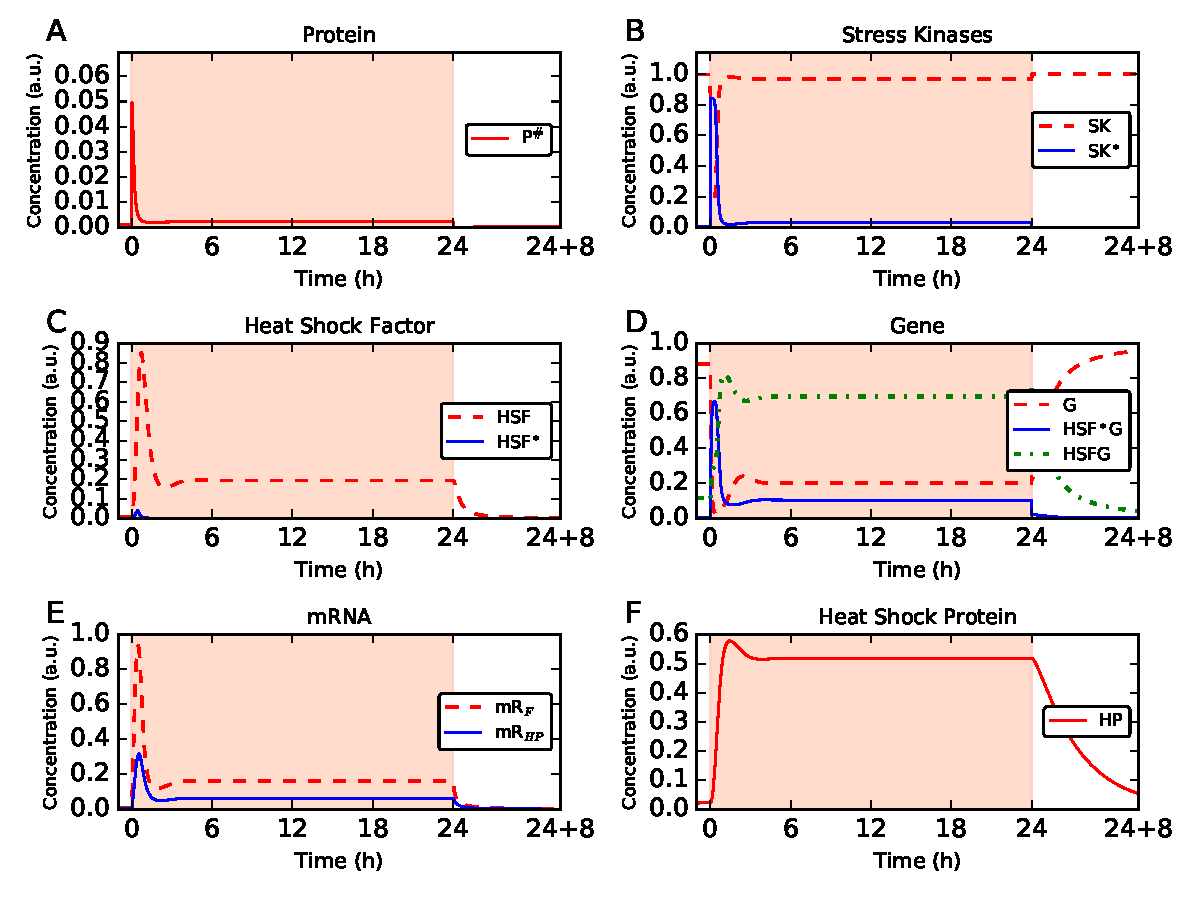
\includegraphics[width=\textwidth, height=0.40\textheight]{HeatShockResponse_SimulationEarlyHSLateHSRecovery.pdf}}
  %\caption*{\small{Simulation of the HSR under long-term HS and recovery.}}
%\endminipage\hfill
%\minipage{0.50\textwidth}
%  \subfloat[Different steady states reached for different temperatures.\label{FigSteadyStadeConcentrations}]{
%  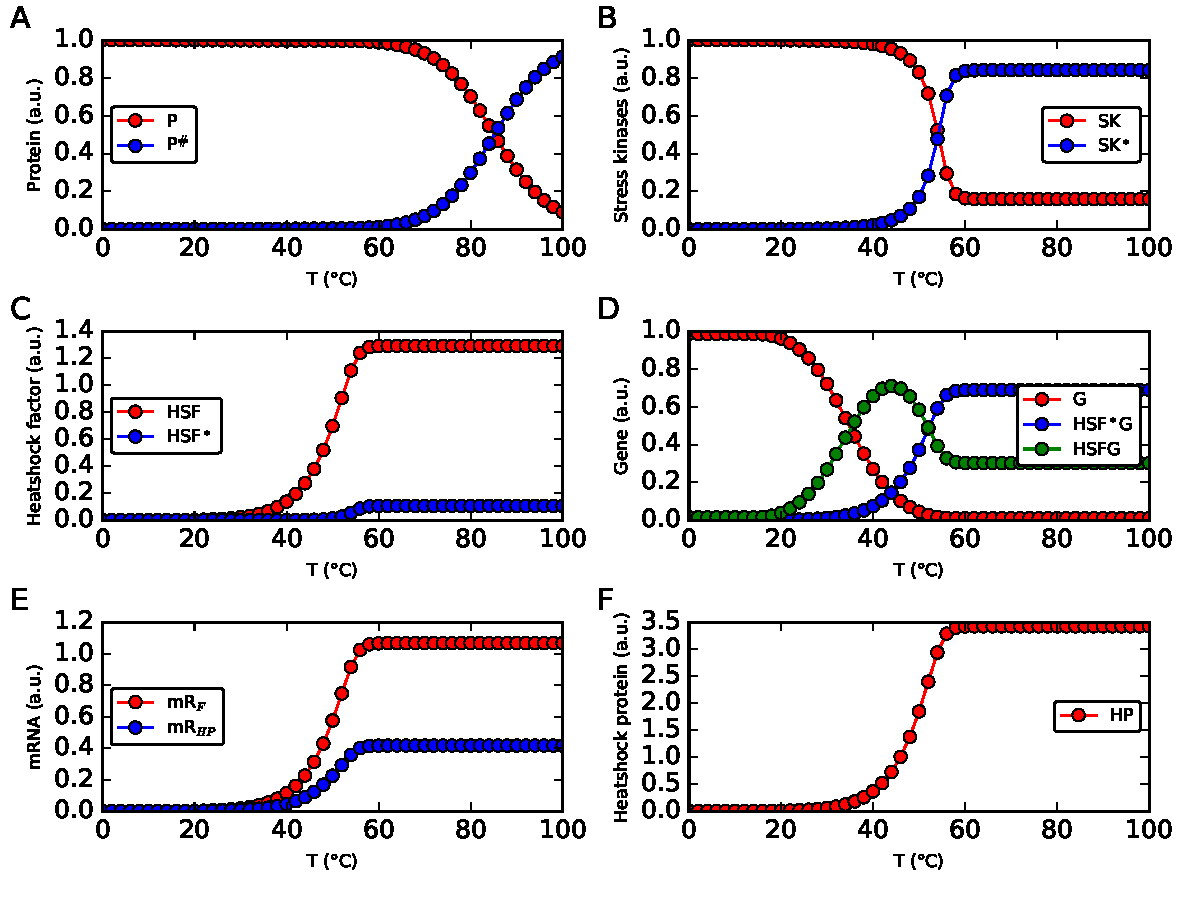
\includegraphics[width=\textwidth, height=0.40\textheight]{EvolutionOfEquilibriumPoint9eqsFuncOfTEMPERATURE.pdf}}
  %\caption*{\small{Different steady states reached for different temperatures.}}
%\endminipage\hfill
%\minipage{1.10\textwidth}
%  \subfloat[Systematic study of the HSP production as a function of different HS temperatures and HS durations.\label{SystematicTdT}]{
%  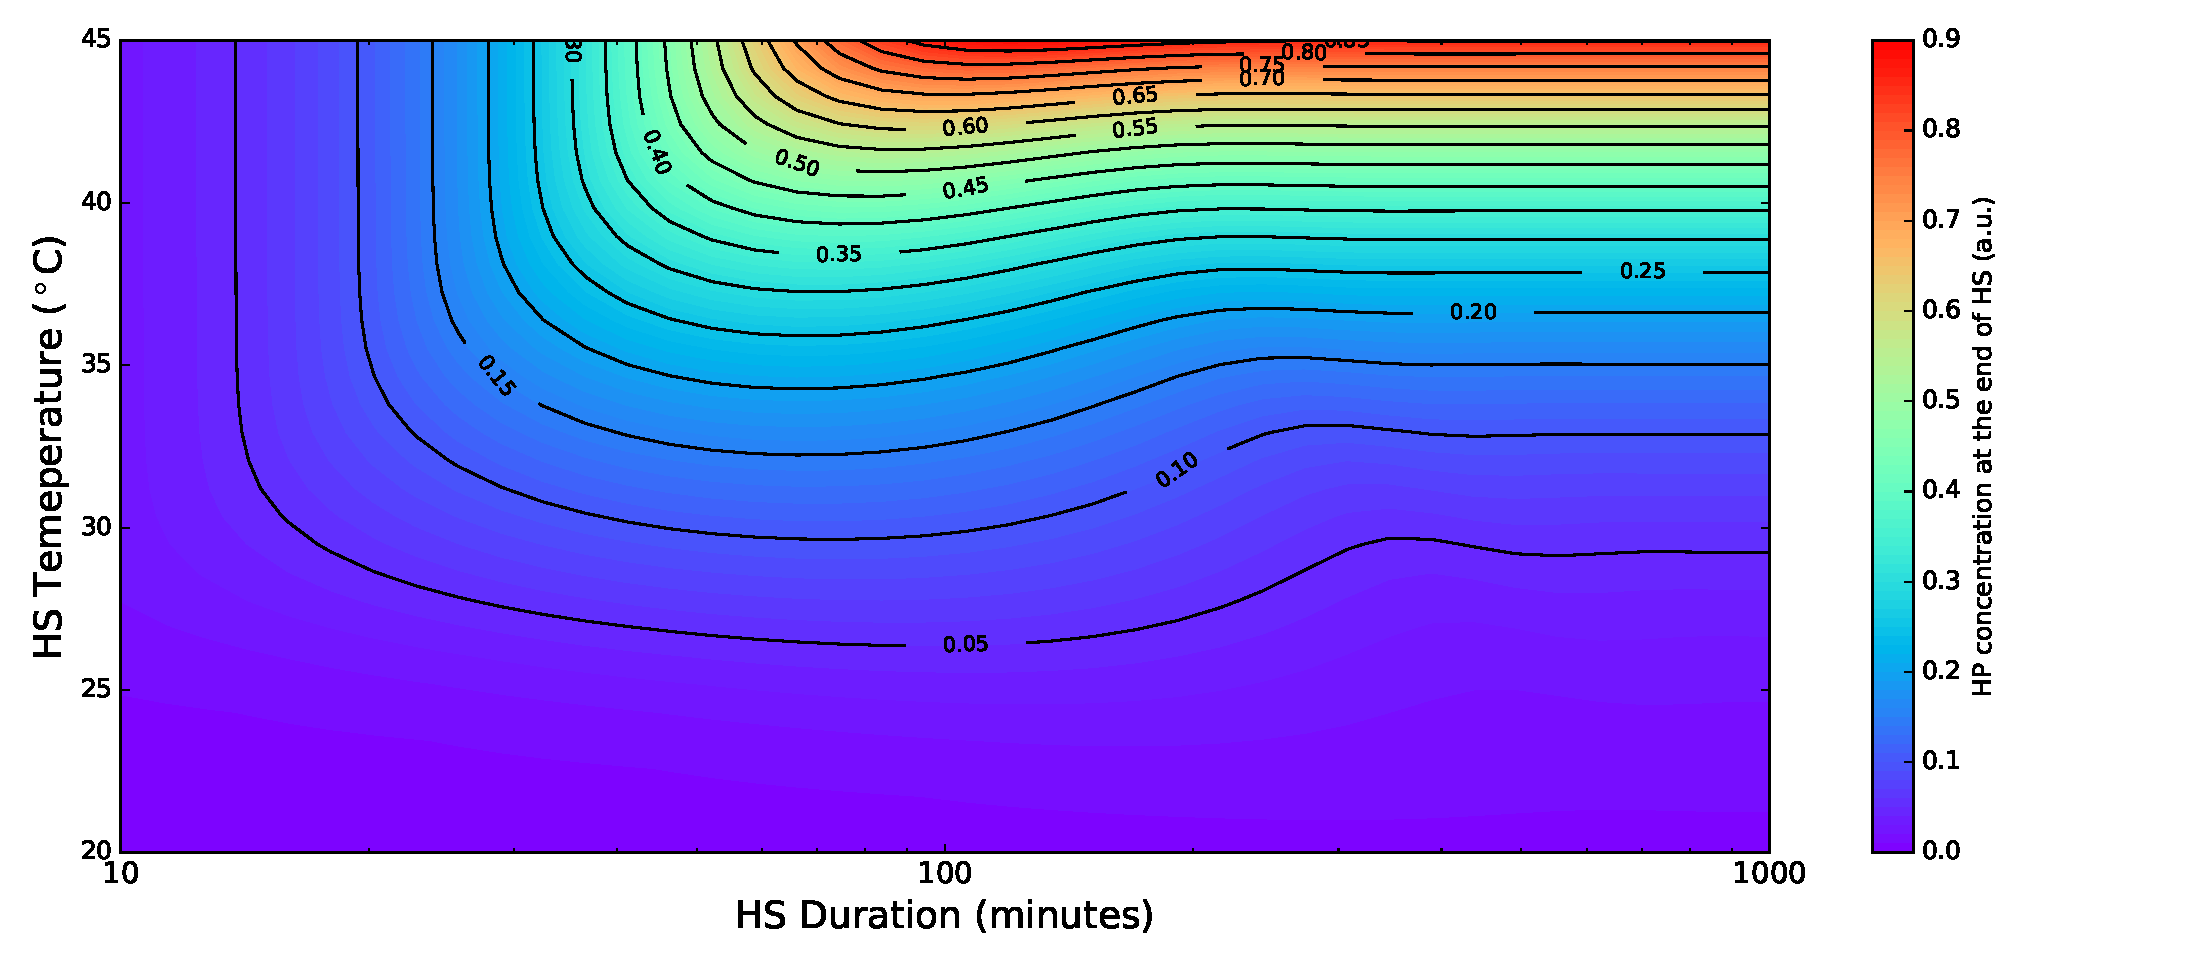
\includegraphics[width=\textwidth, height=0.35\textheight]{ExploreTemperatureDurationHS.pdf}}
  %\caption*{\small{Systematic study of the HSP production as a function of different HS temperatures and HS durations.}}
%\endminipage\hfill
%\caption{\small{Additional results: the organism adapt to long term HS (by reaching a new steady state) but only up to reasonable temperatures. (a) Simulation of the HSR under long-term HS and recovery, provided by shifting the temperature from 25°C to 42°C at $t=0$ and back to 25°C after 24 h. Two distinct phases are clearly visible: an early HS lasting for about the first $3$ h, and a late HS in which the system shows adaptation (a new steady state is reached). 
% The recovery phase is characterized by no urgency to recover the conditions pre-HS at the level of HP.
%After reverting the conditions to normal temperatures (25°C), a recovery phase can be observed, in which
%the variables relax to the original stationary state over a period of several hours. (b) These simulations illustrates how different steady state concentrations are reached for different temperatures. Each point represents the value of the corresponding concentration at the steady state reached for that particular temperature. The concentrations of HP, as well as of the mRNAs, increase with increasing temperature. The concentration of unfolded proteins $\left[P^\#\right]$ is kept very close to zero for low values of the temperature. When the temperature increases considerably the HSR is no more able to efficiently counteract the accumulation of degenerated proteins which accumulates at concentrations high enough to kill the cell. This accumulation is evident in panel A. 
%, a magnification of which is provided in Fig.~\ref{FigSteadyStadeConcentrationsZOOM}. 
%(c) Systematic study of the HSP production as a function of different HS temperatures and HS durations. Short (smaller than $10$ min) HSs do not provide enough time for a significant response at the level of $\left[HP\right]$, the maximum of $\left[HP\right]$ for any given temperature is obtained at around $80$ to $100$ min, after that a somewhat smaller $\left[HP\right]$ is reached and maintained, and for long enough HS a higher temperature provides higher $\left[HP\right]$. From this plot one can understand the trade-off between duration and temperature.}}
%  \label{Figure8label}
%\end{figure*}

\begin{figure*}
\centering
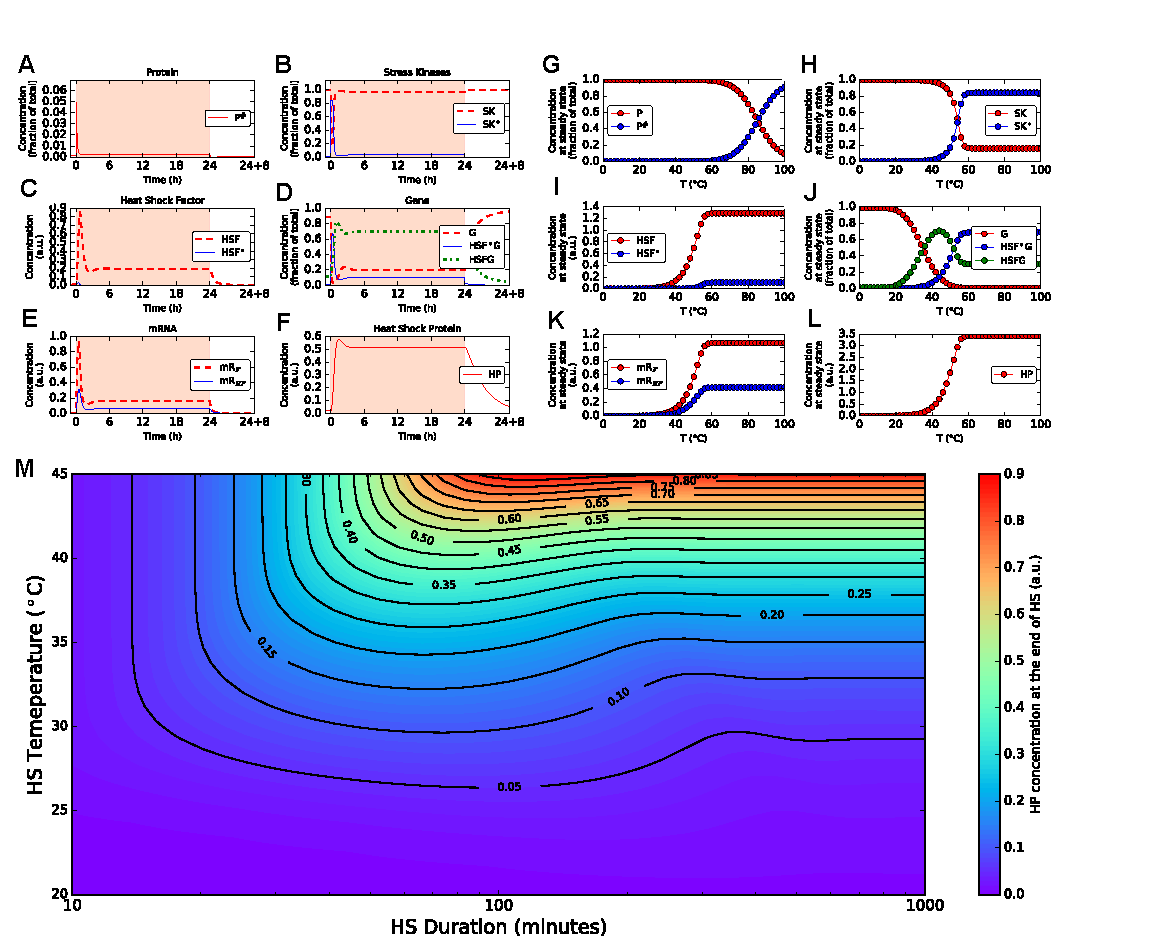
\includegraphics[width=\textwidth]{Figure8_SupMat.pdf}
\caption{\small{\textbf{The organism {acclimates} to long term HS by reaching a new steady state, but only up to reasonable temperatures.} \textbf{(A-F)} Simulation of the HSR under long-term HS and recovery, provided by shifting the temperature from 25°C to 42°C at $t=0$ and back to 25°C after 24 h. Two distinct phases are clearly visible: an early HS lasting for about the first $3$ h, and a late HS in which the system shows {acclimation} (a new steady state is reached). 
% The recovery phase is characterized by no urgency to recover the conditions pre-HS at the level of HP.
After reverting the conditions to normal temperature (25°C), a recovery phase can be observed, in which
the variables relax to the original stationary state over a period of several hours. \textbf{(G-L)} These simulations illustrate how different steady state concentrations are reached for different temperatures. Each point represents the value of the corresponding concentration at the steady state reached for that particular temperature. The concentrations of HP, as well as that of the mRNAs, increase with increasing temperature. The concentration of unfolded proteins $\left[P^\#\right]$ is kept very close to zero for low values of the temperature. When the temperature increases considerably the HSR is no more able to efficiently counteract the accumulation of degenerated proteins which accumulates at concentrations high enough to kill the cell. This accumulation is evident in panel G. Already at about $T \approx $40°C the concentration of accumulated $P^{\#}$ at steady state starts to grow considerably, while above $T \approx $60°C it starts to become overwelming.
%, a magnification of which is provided in Fig.~\ref{FigSteadyStadeConcentrationsZOOM}. 
\textbf{(M)} Systematic study of the HSP production as a function of different HS temperatures and HS durations. Short (smaller than $10$ min) HSs do not provide enough time for a significant response at the level of $\left[HP\right]$, the maximum of $\left[HP\right]$ for any given temperature is obtained at around $80$ to $100$ min, after that a somewhat smaller $\left[HP\right]$ is reached and maintained, and for long enough HS a higher temperature provides higher $\left[HP\right]$. From this plot one can understand {the combined effect of duration and temperature of the HS on the expression of $HSP$.}}
}
\label{Figure8label}
\end{figure*}



\clearpage

\section{{Supplementary Material: Robustness of the main results against changes in Hill kinetics parameters}}
\label{SecRobustness}

{The non-linearity introduced by the Hill kinetics term $\omega_{PS}$ by which the stress kinases $SK$ get activated (Table~\ref{TabNUs}) is crucial to achieve the current model behavior, which would be impossible to achieve with e.g. a linear term. This non-linearity is a critical component necessary for the model to provide the highly sensitive initiation of the heat shock response. On the other hand, the values of the two parameters $m$ and $P_0$ are not that crucial, and thus were not part of the parameter estimation procedure, which involved only the 20 rate constants. Their values were manually set before the fitting procedure, which was then performed with these two parameters fixed at the nominal values of $m=5$ and $P_0=600$ $\mu M$.} 

{To investigate how relevant the values of these two parameters are w.r.t the results which we obtain, and to assess the robustness of our results against changes in $m$ and $P_0$, we perform here additional simulations to show what is the impact of perturbations in these two parameters. We consider the effects on the result of the calibration procedure (Fig.~\ref{Figure2label}~A and Fig.~\ref{Figure2label}~B) on the one hand, and on the main result of this paper, i.e. how the maximum concentration of unfolded protein $P^\#$ during HS depends on how fast the heat shock was applied (Fig.~\ref{Figure4label}~I), on the other hand. These figures are reproposed in Fig.~\ref{Figure9label}~A to simplify the comparison. The value in the green circle in the third panel corresponds to the value of the peak in Fig.~\ref{Figure1label}~B, because the HS of that figure exhibits an increase in temperature which occurs within less then 1 minute. We thus consider the effects produced by variations in the two parameters $m$ and $P_0$ on the simulations reported in panel A. We first consider effects of variations only of $m$, decreasing it, panel~B, or increasing it, panel~C. We then consider the effects of variations only of $P_0$, decreasing it, panel~D, or increasing it, panel~E.
We finally consider the effects of simultaneous variations of both $m$ and $P_0$, aiming at maintaining a low RMS, panel~F.} 

{We clearly see that in all cases the RMS is higher (i.e. worse) than using the original values $m=5$ and $P_0=600$ $\mu M$, due to the fact that these values were kept constant during the fitting of the 20 rate constants to the data. 
As we can see, the qualitative behavior of the maximum concentration of unfolded protein $P^\#$ (right column) in any case does not change significantly, and the switch between the two regimes always occurs in the range between around $1$ $min$ and $100$ $min$ for the duration of the HS onset. Thus our main conclusion, i.e. that the accumulation of unfolded proteins dramatically differs for abrupt (e.g. $< 1$ $min$), or gradual (e.g. $> 100$ $min$) temperature increases, is robust.
One might notice that the value of the maximum concentration of unfolded protein $P^\#$  for short times (values in the circles) changes across half an order of magnitude. While this might seem a lot at a first glance, it should be considered that changes in only one of the two parameters $m$ and $P_0$ lead often to a dramatic increase in the RMS (by far worse than the RMS value corresponding to the final or fiducial parameter set). A low RMS can be achieved for instance by simultaneous changes of both parameters, panel~F. In this case we see that the maximal value of $[P^\#]$ is $0.035$ $\mu M$, close to the original one which was $0.05$ $\mu M$.} 

{To summarize, both parameters could have been included in the fitting procedure, which would have tended to minimize the RMS, but we considered this not necessary. In fact, the drastic difference in accumulated unfolded proteins between sharp and gradual HSs is very robust and occurs for all the variations considered, despite changes in the absolute values of the accumulated unfolded protein. All the parameter changes considered here are anyway discouraged by the calibration data, as the considerably increased RMS obtained in all cases proves.}



\begin{figure*}
\centering
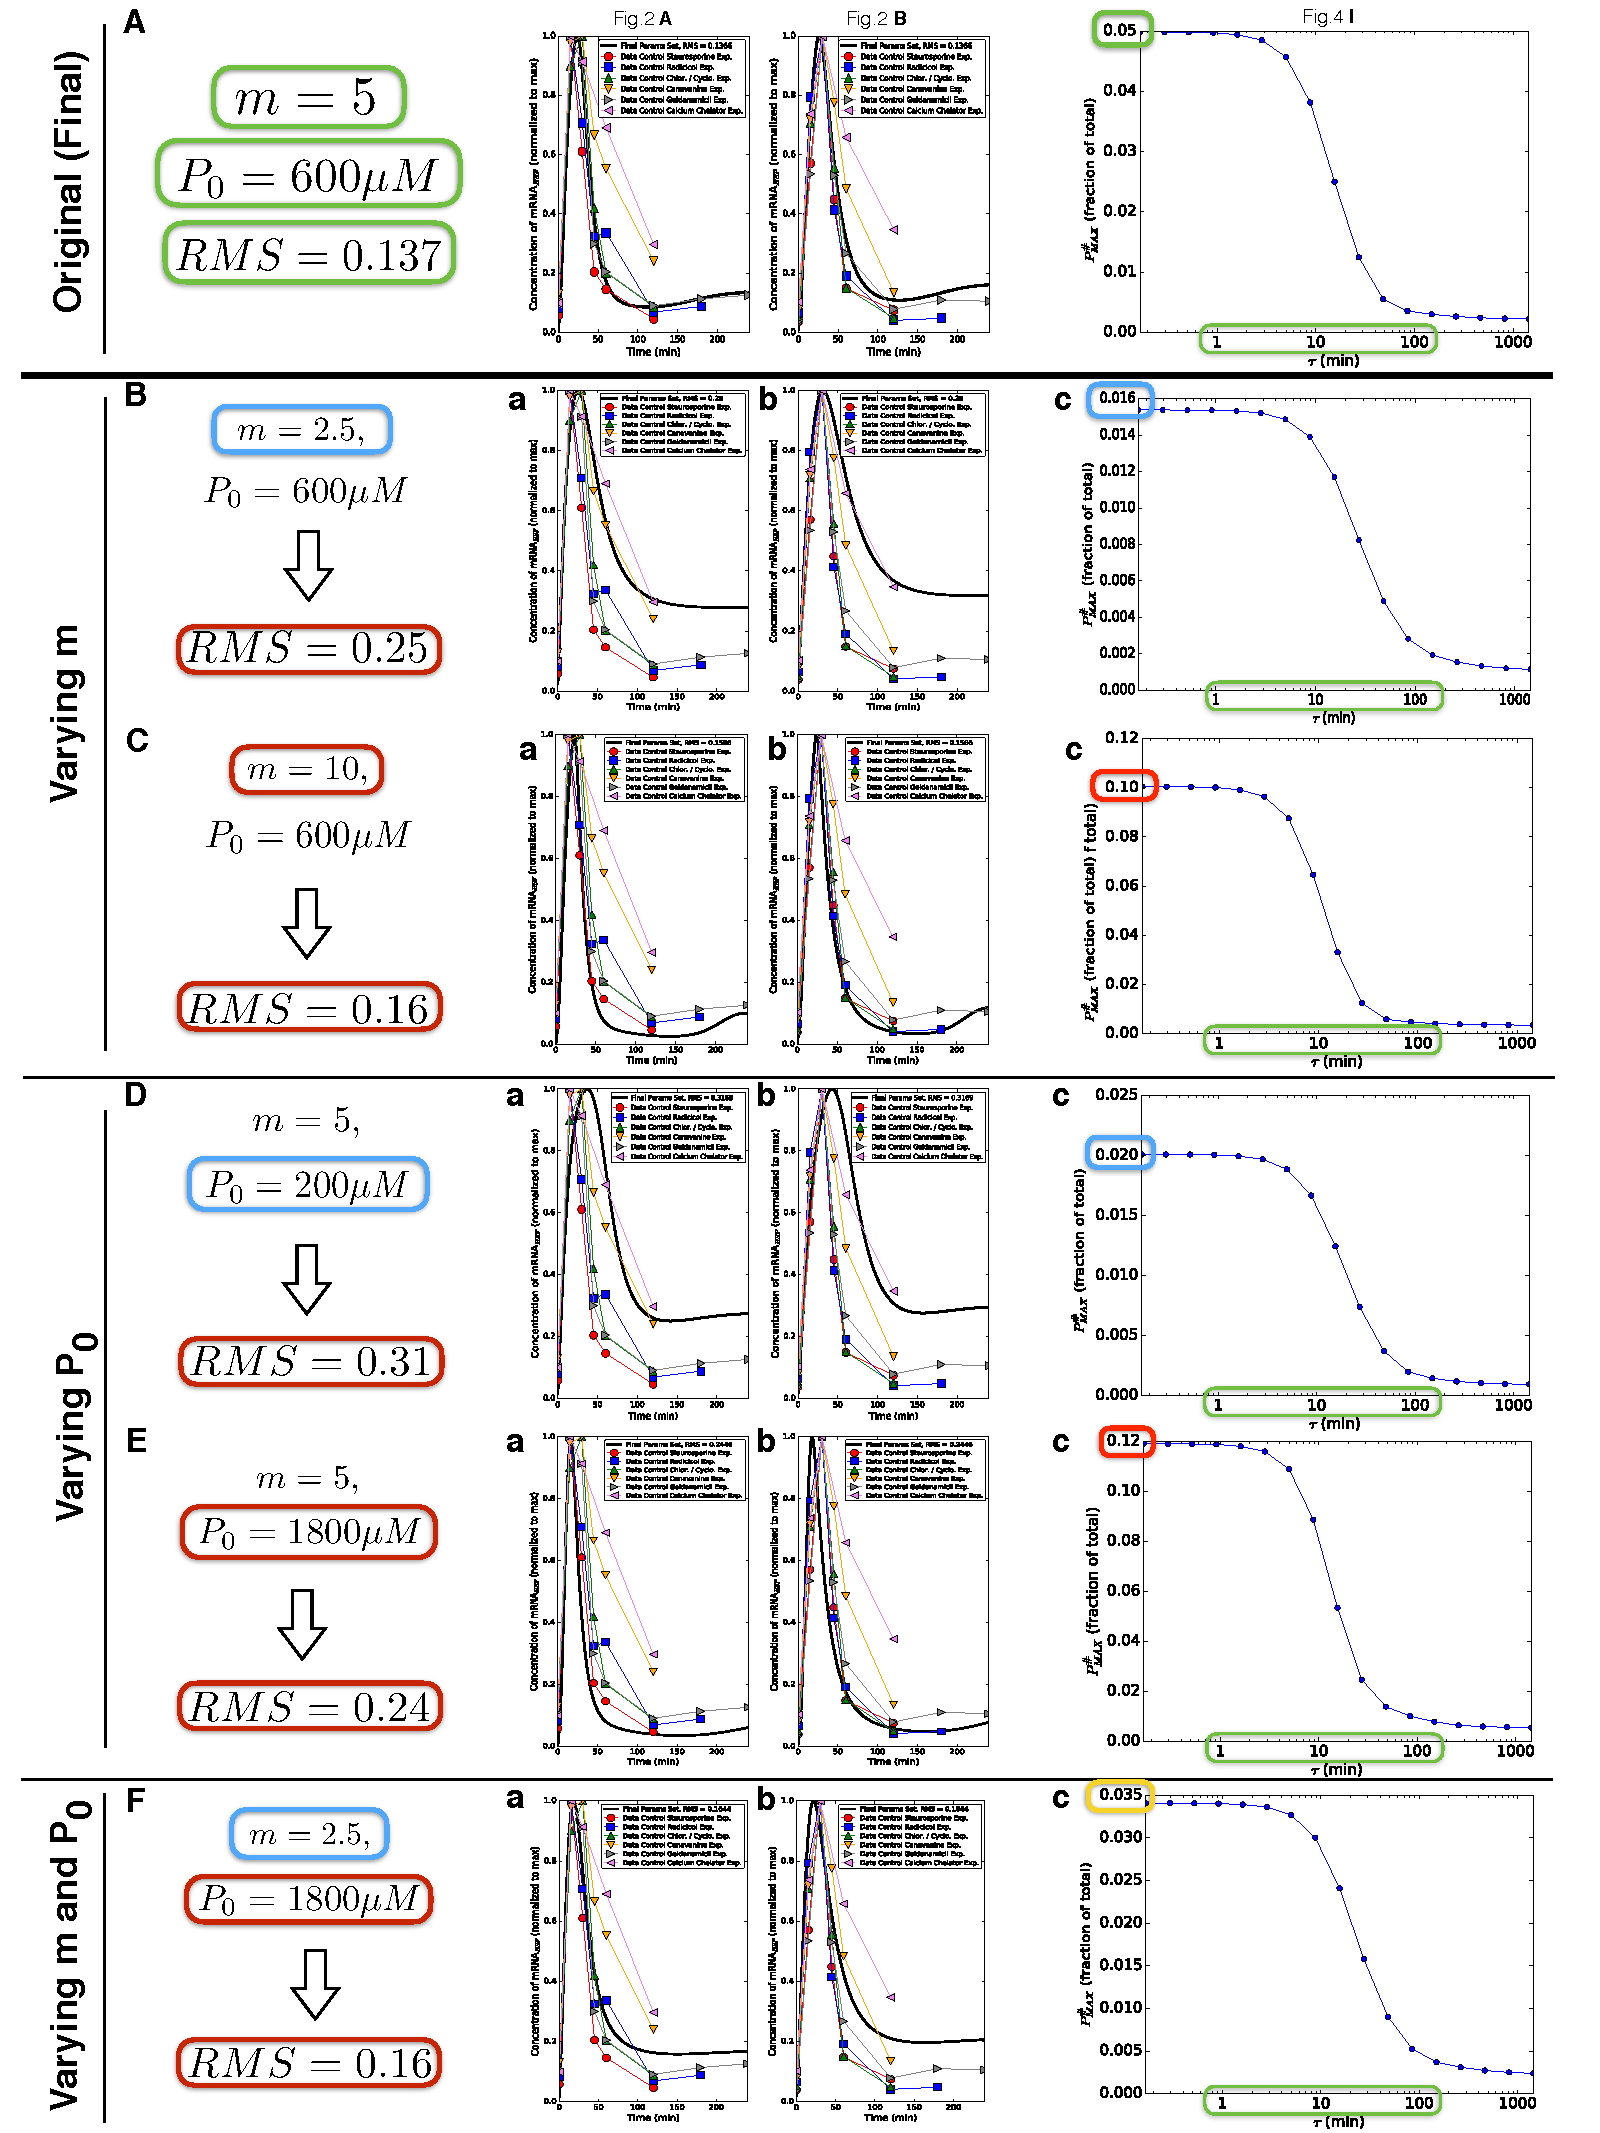
\includegraphics[width=0.77\textwidth]{Figure9_SupMat.pdf}
\caption{\small{{\textbf{Robustness of the results against changes in Hill kinetics parameters.} \textbf{(A)} Calibration data and corresponding model simulations reproposed from Fig.~\ref{Figure2label}~A and Fig.~\ref{Figure2label}~B, and main result on the maximum concentration of unfolded proteins accumulated at steady state reproposed from Fig.~\ref{Figure4label}~I. \textbf{(B,F)} Effects on the simulations of panel A produced by changes in the two parameters $m$ and $P_0$ appearing in the Hill kinetics term $\omega_{PS}$ by which the stress kinease $SK$ gets activated (Table~\ref{TabNUs}). These two parameters where not part of the model fitting procedure but rather manually selected, this figure thus describes the robustness of the result shown in Fig.~\ref{Figure4label}~I against changes in $m$ and $P_0$. \textbf{(B,C)} Effects of variations only of $m$, decreasing it \textbf{(B)} or increasing it \textbf{(C)}. \textbf{(D,E)} Effects of variations only of $P_0$, decreasing it \textbf{(D)} or increasing it \textbf{(E)}. \textbf{(F)} Effects of simultaneous variation of both $m$ and $P_0$, aiming at maintaining a low RMS. The drastic difference in accumulated unfolded proteins between sharp and gradual HSs is very robust and occurs for all the variations considered, despite changes in the absolute values of the accumulated unfolded protein. All the parameter changes considered here are anyway discouraged by the calibration data, as the considerably increased RMS obtained in all cases proves.}}}
\label{Figure9label}
\end{figure*}


\end{document}
